\chapter{Cycles and Continued Fractions}\label{chap:cycles}

The Collatz conjecture\index{Collatz conjecture} asserts two things at once: no orbit of a positive
integer escapes to infinity, and no orbit settles into a cycle other than
$1\mapsto4\mapsto2\mapsto1$. \Cref{chap:intro} called these the divergence
half and the cycle half. The two halves are very different in character. The
divergence half is a statement about the long run behaviour of a single
orbit, and all the probabilistic machinery of the earlier chapters bears on it
only through ensembles. The cycle half is much more rigid. A cycle is a finite
object, it satisfies an exact multiplicative identity, and that identity turns
the question into one about how well the number $\lt$ can be approximated by
rationals.

This chapter develops that reduction completely. We begin with the cycles that
do exist, on the negative integers\index{negative cycles} and on the rationals with odd denominator,
because they show that the cycle identity\index{cycle identity} is not vacuous. We then prove the
identity and its consequence, an upper bound on the least element of a cycle
in terms of the one sided distance from $r\lt$ up to the next integer, where
$r$ is the number of odd elements. To exploit it we need continued fractions\index{continued fraction},
and we give a primer that is complete in itself, including the classical
theorem identifying the best one sided approximations\index{one sided approximation} with the intermediate
fractions of one parity~\cite[Theorem~4.5(ii)]{hancl2019}. The heart of the chapter is a short \emph{mediant
lemma}, a self contained proof of a classical fact, which shows that the first value of $r$ not excluded
by a given verification range\index{verification range} must be a best one sided approximation. This
makes the search for the sharp cycle bound short and rigorous: with the
verification range $2^{68}$, and equally with the current range $2^{71}$, every nontrivial cycle has at least
$72\,057\,431\,991$ odd elements. We compare this with the cruder bounds one
obtains without the lemma, place it in the literature (where sharper
numerical bounds exist and where we claim no priority), and then prove that
no Diophantine\index{Diophantine approximation} argument of this kind can finish the job, a point that Halbeisen\index{Halbeisen, L.} and Hungerb\"uhler\index{Hungerbuhler, N.@Hungerb\"uhler, N.}~\cite[\S5]{halbeisen1997} made earlier in another form (\cref{rem:attribution}): for every
verification range infinitely many $r$ survive. What is missing is arithmetic
information about the parity word, and a window lemma\index{window lemma} makes precise how much
would suffice. We also give an exact integer certificate\index{certificate} for the sharp bound.

Two further sections connect the chapter to recent work. The first treats a
sibling problem of Erd\H{o}s, settled in 2026 by an automated prover, in which
good rational approximations to $\lt$ play the opposite role. The second describes a
small library of machine checked statements in the Lean\index{Lean} proof assistant and
the path from it to a fully verified cycle bound.

Throughout, $\theta=\lt=1.584963\ldots$, $\log$ is the natural logarithm, and we use the three maps of
\cref{def:maps}: the standard map\index{standard map} $T_0$, the accelerated map\index{accelerated map} $T$ and the
Syracuse map\index{Syracuse map} $S$.

\section{The cycles that exist}\label{sec:ch8:exist}

\subsection{The trivial cycle}

The orbit of $1$ is periodic under all three maps: $1\mapsto4\mapsto2\mapsto1$
under $T_0$, $1\mapsto2\mapsto1$ under $T$, and $S(1)=1$. It has one odd
element and two halvings, so in the notation used below $r=1$ and $s=2$, with
period $r+s=3$ under $T_0$, period $s=2$ under $T$ and period $r=1$ under $S$.
The conjecture is that every positive integer eventually enters this cycle;
the cycle half asks only that there be no other.

\subsection{Cycles on the negative integers}

The maps $T_0$, $T$ and $S$ make sense on all of $\Z$, and on the negative
integers there are several cycles. Under $n\mapsto-n$ the standard map\index{standard map} on the
negative integers\index{negative cycles} becomes the map $n\mapsto n/2$ for even $n$ and
$n\mapsto3n-1$ for odd $n$ on the positive integers, the so called $3x-1$
problem, so these cycles are cycles of that problem in disguise. We ran $T_0$
from every starting value $n=-1,-2,\dots,-10^{6}$ and recorded the cycle that
each orbit enters (script \texttt{ch08\_negative.py}). Exactly three cycles
occur, and every one of the $10^6$ starting values falls into one of them.

\begin{table}[ht]
\centering
\caption{The cycles of $T_0$ entered by orbits of $n=-1,\dots,-10^{6}$. Here
$r$ is the number of odd elements and $s$ the number of halvings, so the
period under $T_0$ is $r+s$. The last column counts the starting values that
reach the cycle.}
\label{tab:ch8:negative}
\begin{tabular}{@{}lrrrr@{}}
\toprule
odd elements & $r$ & $s$ & $r+s$ & orbits \\
\midrule
$-1$ & $1$ & $1$ & $2$ & $327\,679$ \\
$-5,-7$ & $2$ & $3$ & $5$ & $323\,351$ \\
$-17,-25,-37,-55,-41,-61,-91$ & $7$ & $11$ & $18$ & $348\,970$ \\
\bottomrule
\end{tabular}
\end{table}

The second cycle is $-5\mapsto-14\mapsto-7\mapsto-20\mapsto-10\mapsto-5$ and
the third, of period $18$ under $T_0$, starts
$-17\mapsto-50\mapsto-25\mapsto-74\mapsto\cdots$. In each case the product of
the factors $3+1/x$ over the odd elements $x$ is an exact power of two: $2$
for the first cycle, $(3-\tfrac15)(3-\tfrac17)=8$ for the second, and $2^{11}$
for the third (we checked the last in exact rational arithmetic). This is the
cycle identity\index{cycle identity} of \cref{lem:cycleid} below. Because the elements are negative
the factors are less than $3$, so $2^s<3^r$, that is, $s<r\theta$: indeed
$3<2\theta=3.17$ and $11<7\theta=11.09$. For positive cycles the inequality
goes the other way, and that change of sign is the whole difficulty. The
negative cycles exist because $2^s$ may undershoot $3^r$ by a little; a
positive cycle would need $2^s$ to overshoot $3^r$ by very little, and the
rest of this chapter quantifies how little.

\subsection{Rational cycles}

Solving the affine identity \eqref{eq:ch2:affine} for a point that returns to itself, as in the proof of \cref{cor:ch2:cycle}, gives, for any parity word $w$ of length $k$ with $m$
ones, the number
\[
  n(w)=\frac{c(w)}{2^k-3^m},
\]
where $c(w)$ is the sum \eqref{eq:ch2:cexplicit}. The identity
\eqref{eq:ch2:affine} holds in the ring of rationals with odd denominator,
in which parity is the parity of the numerator, and reading it backwards shows
that $n(w)$ is a periodic point of $T$ with parity word $w$, repeated. For
example $w=(1,0,0)$ has $c=1$ and $n=1/(8-3)=1/5$, and indeed
$\tfrac15\mapsto\tfrac45\mapsto\tfrac25\mapsto\tfrac15$. Every word thus gives
a rational cycle\index{rational cycles}, and the integer cycles are exactly the words for which
$2^k-3^m$ divides $c(w)$. Lagarias\index{Lagarias, J. C.}~\cite{lagarias1990} studied the set of
these rational cycles systematically, organizing them by denominator; for a
denominator $d$ coprime to $6$ they correspond to the integer cycles, with elements prime to $d$, of the map that sends $x$ to $(3x+d)/2$ for odd $x$ and to $x/2$ for even $x$, and he showed, among other things, that cycles exist for many denominators. We shall not need this theory. Its lesson for us is that
there is no shortage of periodic parity words; what is rare is the
divisibility that makes $n(w)$ an integer, and for positive integers the
inequality $3^m<2^k$ of \cref{cor:ch2:cycle} combined with the size of the
elements is the only handle we have.

\section{The cycle identity}\label{sec:ch8:identity}

It is most convenient to describe a cycle by its odd elements. Suppose $S$ has
a cycle of positive odd integers $x_1,\dots,x_r$, with $x_{i+1}=S(x_i)$
(indices modulo $r$), and let $k_i=\vt(3x_i+1)\geq1$ be the halving exponents,
so that
\begin{equation}\label{eq:ch8:stride}
  x_{i+1}=\frac{3x_i+1}{2^{k_i}} .
\end{equation}
Put $s=\sum_i k_i$, the total number of halvings in one turn of the cycle.

\begin{lemma}[Cycle identity]\label{lem:cycleid}
For a cycle of $S$ as above,
\begin{equation}\label{eq:ch8:prod}
  \prod_{i=1}^{r}\Bigl(3+\frac{1}{x_i}\Bigr)=2^{s},
\end{equation}
and therefore, writing $M=\min_i x_i$ for the least element,
\begin{equation}\label{eq:ch8:Lambda}
  \Lambda:=s\log2-r\log3=\sum_{i=1}^{r}\log\Bigl(1+\frac{1}{3x_i}\Bigr)
  \in\Bigl(0,\ \frac{r}{3M}\Bigr).
\end{equation}
Equivalently,
\begin{equation}\label{eq:ch8:theta}
  0<s-r\theta<\frac{r}{3M\log2},
\end{equation}
and in particular $s/r>\theta$.
\end{lemma}

\begin{proof}
Multiply the $r$ relations \eqref{eq:ch8:stride} around the cycle. The
product of the left sides is $\prod_ix_i$ and the product of the right sides
is $\prod_i(3x_i+1)/2^{s}$, so $2^s=\prod_i(3x_i+1)/x_i$, which is
\eqref{eq:ch8:prod}. Taking logarithms and writing
$\log(3+1/x_i)=\log3+\log(1+1/(3x_i))$ gives the middle expression in
\eqref{eq:ch8:Lambda}. Each summand is positive, so $\Lambda>0$, and since
$\log(1+u)<u$ for $u>0$ and $1/(3x_i)\leq1/(3M)$, we get
$\Lambda<r/(3M)$.
Dividing by $\log2$ gives \eqref{eq:ch8:theta}.
\end{proof}

The same identity can be read off from the affine form of
\cref{prop:ch2:affine}. If $n$ is an element of a cycle of $T$ of length $k$
with $m$ odd steps, then \eqref{eq:ch2:product} with $T^{(k)}(n)=n$ says that
$2^k/3^m$ is the product of $1+1/(3y)$ over the odd elements $y$ of the cycle.
That is \eqref{eq:ch8:prod} with $m=r$ and $k=s$.

\begin{remark}[A pitfall: bookkeeping under the accelerated map]\label{rem:ch8:bookkeeping}
The three maps count the same cycle differently, and it is easy to mix the
counts. Under the Syracuse map\index{Syracuse map} $S$ the cycle has period $r$. Under the
accelerated map\index{accelerated map} $T$ each odd step already contains one halving, so the cycle
has $s$ steps in all, of which $r$ are odd and $s-r$ are even. Under the
standard map\index{standard map} $T_0$ every halving is a separate step and so is every tripling,
so the period is $r+s$. For the trivial cycle these are $1$, $2$ and $3$.
The linear form can be written either as $s\log2-r\log3$ or as
$s'\log2-r\log(3/2)$ with $s'=s-r$ the number of even steps of $T$, and the
two are equal. The danger lies in the derived quantities. If one works with
$s'$ and then reports $s'$, or $s$, as ``the period'' of the cycle, the
answer is wrong for $T_0$, whose period is $r+s=2r+s'$. And the feasibility
condition must be stated for the right pair: it is $s/r>\theta$, equivalently
$s'/r>\theta-1=\log_2(3/2)$, together with the constraint $s'\geq0$ that
comes from $k_i\geq1$. Lower bounds on cycle length in the literature are
quoted in all three conventions, and comparisons between them are meaningless
unless the convention is fixed. In this chapter $r$ is the number of odd
elements and $s$ the number of halvings, so that a cycle has $r$ steps of
$S$, $s$ steps of $T$ (of which $r$ are odd) and $r+s$ steps of $T_0$.
\end{remark}

For fixed $r$ the strongest conclusion comes from the smallest admissible
$\Lambda$. Since $s$ must be an integer with $s>r\theta$, we have
$s\geq\lceil r\theta\rceil$ and so
\begin{equation}\label{eq:ch8:Lambdar}
  \Lambda\geq\Lambda_r:=\delta(r)\log2,\qquad
  \delta(r):=\lceil r\theta\rceil-r\theta\in(0,1).
\end{equation}
(The value $\delta(r)$ is never $0$ because $\theta$ is irrational: $2^s=3^r$
is impossible for $r\geq1$.) Combining with \eqref{eq:ch8:Lambda} gives the
basic inequality of the chapter:
\begin{equation}\label{eq:ch8:maxM}
  M<\frac{r}{3\Lambda_r}=\frac{r}{3\,\delta(r)\log2}=:F(r).
\end{equation}
The function $F$ depends only on $\theta$ and $r$. A cycle with $r$ odd
elements must have its least element below $F(r)$. On the other hand, if
every positive integer up to some bound reaches $1$, then every element of a
nontrivial cycle exceeds that bound. These two facts squeeze the cycle.

\begin{definition}[Verification range and exclusion]\label{def:ch8:excl}
We say that $X$ is a \emph{verified range\index{verification range}} if every element of every
nontrivial cycle of positive integers is at least $X$; this holds, for
example, if every positive integer $n<X$ is known to reach $1$. Given $X$, put
$\varepsilon=\varepsilon(X)=1/(3X\log2)$ and say that $r\geq1$ is
\emph{excluded} if $\delta(r)\geq r\varepsilon$, equivalently $F(r)\leq X$.
\end{definition}

\begin{corollary}\label{cor:ch8:excl}
If $X$ is a verified range, then a nontrivial cycle with $r$ odd elements
satisfies $\delta(r)<r\varepsilon$, so $r$ is not excluded.
\end{corollary}

\begin{proof}
By \eqref{eq:ch8:theta}, $\delta(r)\leq s-r\theta<r/(3M\log2)\leq
r/(3X\log2)=r\varepsilon$.
\end{proof}

By Ba\v{r}ina\index{Barina, D.@Ba\v{r}ina, D.}~\cite{barina2021}, every positive integer below $2^{68}$
reaches $1$, so $X=2^{68}=2.95148\times10^{20}$ is a verified range. Ba\v{r}ina~\cite{barina2025} has since extended the verification to $2^{71}$; we keep $X=2^{68}$ in the examples, and \cref{sec:ch8:bound} shows that the larger range gives the same sharp bound. The
question is now purely arithmetic: which $r$ satisfy $\delta(r)<r\varepsilon$?
The inequality says that $r\theta$ lies just \emph{below} an integer, closer
than $r\varepsilon$. To find all such $r$ we need the theory of rational
approximation, and specifically its one sided form.

\section{A primer on continued fractions}\label{sec:ch8:cf}

This section collects what we need about continued fractions\index{continued fraction}, with proofs.
The material is classical; good references are the books of
Khinchin\index{Khinchin, A. Ya.}~\cite{khinchin1964}, Hardy\index{Hardy, G. H.} and Wright\index{Wright, E. M.}~\cite{hardywright2008} and
Rockett\index{Rockett, A. M.} and Sz\"usz\index{Szusz, P.@Sz\"usz, P.}~\cite{rockett1992}, the last of which treats one sided
approximation in detail.

\subsection{Convergents and their recurrences}

Let $\theta>0$ be irrational. Define $\theta_0=\theta$ and, recursively,
$a_k=\lfloor\theta_k\rfloor$ and $\theta_{k+1}=1/(\theta_k-a_k)>1$. Then
$a_0\geq0$, $a_k\geq1$ for $k\geq1$, and for every $k$
\[
  \theta=a_0+\cfrac{1}{a_1+\cfrac{1}{\ddots+\cfrac{1}{a_k+\cfrac{1}{\theta_{k+1}}}}}
  =:[a_0;a_1,\dots,a_k,\theta_{k+1}].
\]
The numbers $a_k$ are the \emph{partial quotients} and $\theta_k$ the
\emph{complete quotients}. Define integers $p_k,q_k$ by
\begin{equation}\label{eq:ch8:recur}
  \begin{gathered}
  p_k=a_kp_{k-1}+p_{k-2},\qquad q_k=a_kq_{k-1}+q_{k-2},\\
  p_{-2}=0,\quad p_{-1}=1,\quad q_{-2}=1,\quad q_{-1}=0 .
  \end{gathered}
\end{equation}
Thus $p_0=a_0$, $q_0=1$, $q_1=a_1$, and $1=q_0\leq q_1<q_2<q_3<\cdots$. The
fractions $p_k/q_k$ are the \emph{convergents\index{convergent}}.

\begin{lemma}[Basic identities]\label{lem:ch8:basic}
For every $k\geq0$:
\begin{enumerate}[label=(\roman*),leftmargin=2em]
\item $\begin{pmatrix}a_0&1\\1&0\end{pmatrix}\cdots
  \begin{pmatrix}a_k&1\\1&0\end{pmatrix}
  =\begin{pmatrix}p_k&p_{k-1}\\q_k&q_{k-1}\end{pmatrix}$;
\item $p_kq_{k-1}-p_{k-1}q_k=(-1)^{k-1}$, and this also holds for $k=-1$;
\item $\theta=\dfrac{\theta_{k+1}p_k+p_{k-1}}{\theta_{k+1}q_k+q_{k-1}}$;
\item $q_k\theta-p_k=\dfrac{(-1)^k}{\theta_{k+1}q_k+q_{k-1}}$. In particular
  $p_k/q_k<\theta$ for even $k$ and $p_k/q_k>\theta$ for odd $k$, and the
  error $\varepsilon_k:=|q_k\theta-p_k|$ satisfies
  \[
    \frac{1}{q_{k+1}+q_k}<\varepsilon_k<\frac{1}{q_{k+1}};
  \]
\item $\varepsilon_{k+1}=\varepsilon_{k-1}-a_{k+1}\varepsilon_k$, where
  $\varepsilon_{-1}=|q_{-1}\theta-p_{-1}|=1$.
\end{enumerate}
\end{lemma}

\begin{proof}
(i) is induction on $k$ using \eqref{eq:ch8:recur}, since multiplying the
matrix
$\bigl(\begin{smallmatrix}p_{k-1}&p_{k-2}\\q_{k-1}&q_{k-2}\end{smallmatrix}\bigr)$
on the right by
$\bigl(\begin{smallmatrix}a_k&1\\1&0\end{smallmatrix}\bigr)$ gives
$\bigl(\begin{smallmatrix}p_k&p_{k-1}\\q_k&q_{k-1}\end{smallmatrix}\bigr)$.
(ii) Take determinants in (i): each factor has determinant $-1$; for $k=-1$,
$p_{-1}q_{-2}-p_{-2}q_{-1}=1$.
(iii) The matrix
$\bigl(\begin{smallmatrix}a&1\\1&0\end{smallmatrix}\bigr)$ acts on $t$ as the
M\"obius map $t\mapsto a+1/t$, and composition of M\"obius maps corresponds to
matrix multiplication, so by (i) the map
$t\mapsto[a_0;a_1,\dots,a_k,t]$ is
$t\mapsto(tp_k+p_{k-1})/(tq_k+q_{k-1})$; put $t=\theta_{k+1}$.
(iv) From (iii),
$q_k\theta-p_k=(q_kp_{k-1}-p_kq_{k-1})/(\theta_{k+1}q_k+q_{k-1})$, and the
numerator is $(-1)^k$ by (ii). Since $a_{k+1}<\theta_{k+1}<a_{k+1}+1$, the
denominator lies strictly between $a_{k+1}q_k+q_{k-1}=q_{k+1}$ and
$q_{k+1}+q_k$.
(v) Multiply the recurrence \eqref{eq:ch8:recur} at index $k+1$ by $\theta$
and subtract: $q_{k+1}\theta-p_{k+1}=a_{k+1}(q_k\theta-p_k)+
(q_{k-1}\theta-p_{k-1})$. By (iv), and for $k=0$ by $q_{-1}\theta-p_{-1}=-1$,
the outer two terms have the same sign and the middle one the opposite sign,
which gives the stated relation between absolute values.
\end{proof}

\subsection{Best approximation}

Write $\|t\|$ for the distance from $t$ to the nearest integer. The next
theorem, due in essence to Lagrange\index{Lagrange, J. L.}, is the best approximation property: no
denominator smaller than $q_{k+1}$ approximates $\theta$ better than $q_k$.

\begin{theorem}[Best approximation]\label{thm:ch8:best}
Let $k\geq0$, $1\leq r<q_{k+1}$ and $s\in\Z$. Then
$|r\theta-s|\geq\varepsilon_k$. In particular $\|r\theta\|\geq\varepsilon_k
\geq\|q_k\theta\|$.
\end{theorem}

\begin{proof}
By \cref{lem:ch8:basic}(ii) the matrix
$\bigl(\begin{smallmatrix}p_k&p_{k+1}\\q_k&q_{k+1}\end{smallmatrix}\bigr)$
has determinant $\pm1$, so there are integers $x,y$ with $s=xp_k+yp_{k+1}$ and
$r=xq_k+yq_{k+1}$. Then
$r\theta-s=x(q_k\theta-p_k)+y(q_{k+1}\theta-p_{k+1})$. If $y=0$ then
$r=xq_k$ with $x\geq1$, and $|r\theta-s|=x\varepsilon_k\geq\varepsilon_k$. If
$x=0$ then $r=yq_{k+1}$, which is impossible for $1\leq r<q_{k+1}$. If $x$
and $y$ are both positive then $r\geq q_k+q_{k+1}>q_{k+1}$, and if both are
negative then $r<0$; both are impossible. So $x$ and $y$ are nonzero with
opposite signs. Since $q_k\theta-p_k$ and $q_{k+1}\theta-p_{k+1}$ also have
opposite signs, by \cref{lem:ch8:basic}(iv), the two terms
$x(q_k\theta-p_k)$ and $y(q_{k+1}\theta-p_{k+1})$ have the same sign, and
$|r\theta-s|\geq|x|\varepsilon_k\geq\varepsilon_k$.
\end{proof}

\subsection{Intermediate fractions}

Between two convergents\index{convergent} on the same side of $\theta$ one may interpolate. For
$k\geq0$ and $0\leq j\leq a_{k+1}$ define
\begin{equation}\label{eq:ch8:rung}
  u_{k,j}=q_{k-1}+jq_k,\qquad P_{k,j}=p_{k-1}+jp_k .
\end{equation}
For $j=0$ this is the convergent $p_{k-1}/q_{k-1}$, for $j=a_{k+1}$ it is
$p_{k+1}/q_{k+1}$, and the fractions $P_{k,j}/u_{k,j}$ with $0<j<a_{k+1}$
are the \emph{intermediate fractions\index{semiconvergent}}, or \emph{semiconvergents}. We call the
denominators $u_{k,j}$ the \emph{rungs} of the \emph{semiconvergent ladder}:
the ladder from $q_{k-1}$ to $q_{k+1}$ climbs in steps of $q_k$,
\[
  q_{k-1},\ q_{k-1}+q_k,\ q_{k-1}+2q_k,\ \dots,\ q_{k-1}+a_{k+1}q_k=q_{k+1}.
\]
By \cref{lem:ch8:basic}(iv) and (v),
\begin{equation}\label{eq:ch8:rungerr}
  P_{k,j}-u_{k,j}\theta=(-1)^{k}\bigl(\varepsilon_{k-1}-j\varepsilon_k\bigr),
  \qquad \varepsilon_{k-1}-j\varepsilon_k\geq\varepsilon_{k+1}>0,
\end{equation}
so every rung of the ladder from $q_{k-1}$ lies on the same side of $\theta$
as $p_{k-1}/q_{k-1}$, and the error decreases linearly in $j$. For even $k$
the ladder approximates $\theta$ from above, for odd $k$ from below.

\subsection{One sided best approximation}

For the cycle problem the relevant quantity is the one sided distance
$\delta(r)=\lceil r\theta\rceil-r\theta$ of \eqref{eq:ch8:Lambdar}, the
distance from $r\theta$ up to the next integer. It is small when $s/r$, with
$s=\lceil r\theta\rceil$, approximates $\theta$ well \emph{from above}.

\begin{definition}[One sided records]\label{def:ch8:records}
We call $r\geq1$ a \emph{$\delta$ record}, or a best one sided approximation\index{one sided approximation}
from above, if $\delta(r)<\delta(r')$ for every $1\leq r'<r$.
\end{definition}

\begin{theorem}[One sided best approximations]\label{thm:ch8:onesided}
The $\delta$ records are exactly the rungs $u_{k,j}=q_{k-1}+jq_k$ with $k\geq0$
even and $1\leq j\leq a_{k+1}$. For such a rung,
$\lceil u_{k,j}\theta\rceil=P_{k,j}$ and
$\delta(u_{k,j})=\varepsilon_{k-1}-j\varepsilon_k$.
\end{theorem}

This classical fact is the one sided analogue of \cref{thm:ch8:best}; Han\v{c}l\index{Hancl, J.@Han\v{c}l, J.} and Turek\index{Turek, O.}~\cite[Theorem~4.5(ii)]{hancl2019} give a statement with proof, and
Rockett and Sz\"usz~\cite{rockett1992} treat the theory of one sided
approximation. The same proof with the roles of the parities exchanged shows
that the best approximations from below are $r=1$ and the rungs with $k\geq1$ odd. We give
the short proof, since the whole sharp bound rests on it.

\begin{proof}
Fix an even $k\geq0$ and $0\leq j<a_{k+1}$, and write $u=u_{k,j}$,
$P=P_{k,j}$, $e=P-u\theta$ and $d=\varepsilon_k=q_k\theta-p_k>0$ (positive
because $k$ is even). By \eqref{eq:ch8:rungerr}, $e=\varepsilon_{k-1}-jd>0$.
We claim that
\begin{equation}\label{eq:ch8:claim}
  1\leq r<u+q_k,\ r\neq u\quad\Longrightarrow\quad\delta(r)>e .
\end{equation}
The matrix
$\bigl(\begin{smallmatrix}P&p_k\\u&q_k\end{smallmatrix}\bigr)$ has
determinant $p_{k-1}q_k-p_kq_{k-1}=(-1)^k=1$, so for $s=\lceil r\theta\rceil$
there are integers $x,y$ with $s=xP+yp_k$ and $r=xu+yq_k$, and then
\[
  \delta(r)=s-r\theta=xe-yd\in(0,1).
\]
If $x\leq0$ then positivity of $xe-yd$ forces $y<0$, and then $r=xu+yq_k<0$,
which is impossible. So $x\geq1$. If also $y\geq1$ then $r\geq u+q_k$,
excluded by hypothesis. Hence $y\leq0$ and $\delta(r)=xe+|y|d\geq e$, with
equality only when $x=1$ and $y=0$, that is $r=u$. This proves
\eqref{eq:ch8:claim}.

Now suppose $u\geq1$ (this excludes only $k=0$, $j=0$, where $u=q_{-1}=0$).
Then $e<1$: for $k=0$, $e=1-j\varepsilon_0<1$ since $j\geq1$, and for $k\geq2$,
$e\leq\varepsilon_{k-1}<1/q_k\leq1$. As $e\in(0,1)$ and $P-u\theta=e$, we have
$\lceil u\theta\rceil=P$ and $\delta(u)=e$. By \eqref{eq:ch8:claim}, every
$r<u$ has $\delta(r)>\delta(u)$, so $u$ is a $\delta$ record, and every $r$
with $u<r<u+q_k$ has $\delta(r)>\delta(u)$ with $u<r$, so $r$ is not a
$\delta$ record. The rung $u+q_k=u_{k,j+1}$ is covered by the case $j+1$ if
$j+1<a_{k+1}$, and if $j+1=a_{k+1}$ it equals $q_{k+1}=u_{k+2,0}$, the first
rung of the next ladder, which is covered with $k+2$ in place of $k$ and
$j=0$. The half open intervals $[u_{k,j},u_{k,j}+q_k)$, over even $k$ and
$0\leq j<a_{k+1}$, therefore tile $[0,\infty)$, their left endpoints other
than $0$ are $\delta$ records, and no other integer is. The left endpoints
other than $0$ are precisely the $u_{k,j}$ with $k$ even and $1\leq j\leq
a_{k+1}$ (the endpoint $u_{k+2,0}=u_{k,a_{k+1}}$ being counted once).
\end{proof}

\subsection{The continued fraction of $\lt$}

We computed the partial quotients of $\theta=\lt$ at $300$ significant digits
and confirmed the first $60$ of them at $150$ digits (script
\texttt{ch08\_compute.py}):
\[
  \lt=[1;1,1,2,2,3,1,5,2,23,2,2,1,1,55,1,4,3,1,1,15,1,\dots].
\]
The convergents\index{convergent} are listed in \cref{tab:ch8:conv}. The two large partial
quotients $a_9=23$ and $a_{14}=55$ produce unusually good approximations, at
$q_8=665$ and $q_{13}=190\,537$ respectively; note that the good approximation
at $q_8$ is from below and that at $q_{13}$ from above, a distinction that
will matter.

\begin{table}[ht]
\centering
\caption{Convergents $p_k/q_k$ of $\theta=\lt$. The side column records
whether $p_k/q_k$ lies below or above $\theta$; the last column is
$\varepsilon_k=|q_k\theta-p_k|$.}
\label{tab:ch8:conv}
\small
\begin{tabular}{@{}rrrrlr@{}}
\toprule
$k$ & $a_k$ & $p_k$ & $q_k$ & side & $\varepsilon_k$ \\
\midrule
 0 & 1 & 1 & 1 & below & $0.585$ \\
 1 & 1 & 2 & 1 & above & $0.415$ \\
 2 & 1 & 3 & 2 & below & $0.170$ \\
 3 & 2 & 8 & 5 & above & $7.52\times10^{-2}$ \\
 4 & 2 & 19 & 12 & below & $1.96\times10^{-2}$ \\
 5 & 3 & 65 & 41 & above & $1.65\times10^{-2}$ \\
 6 & 1 & 84 & 53 & below & $3.01\times10^{-3}$ \\
 7 & 5 & 485 & 306 & above & $1.47\times10^{-3}$ \\
 8 & 2 & 1054 & 665 & below & $6.30\times10^{-5}$ \\
 9 & 23 & 24727 & 15601 & above & $2.62\times10^{-5}$ \\
10 & 2 & 50508 & 31867 & below & $1.05\times10^{-5}$ \\
11 & 2 & 125743 & 79335 & above & $5.29\times10^{-6}$ \\
12 & 1 & 176251 & 111202 & below & $5.19\times10^{-6}$ \\
13 & 1 & 301994 & 190537 & above & $9.31\times10^{-8}$ \\
14 & 55 & 16785921 & 10590737 & below & $7.55\times10^{-8}$ \\
15 & 1 & 17087915 & 10781274 & above & $1.76\times10^{-8}$ \\
16 & 4 & 85137581 & 53715833 & below & $5.01\times10^{-9}$ \\
17 & 3 & 272500658 & 171928773 & above & $2.58\times10^{-9}$ \\
18 & 1 & 357638239 & 225644606 & below & $2.43\times10^{-9}$ \\
19 & 1 & 630138897 & 397573379 & above & $1.53\times10^{-10}$ \\
20 & 15 & 9809721694 & 6189245291 & below & $1.38\times10^{-10}$ \\
21 & 1 & 10439860591 & 6586818670 & above & $1.46\times10^{-11}$ \\
22 & 9 & 103768467013 & 65470613321 & below & $6.65\times10^{-12}$ \\
23 & 2 & 217976794617 & 137528045312 & above & $1.30\times10^{-12}$ \\
\bottomrule
\end{tabular}
\end{table}

By \cref{thm:ch8:onesided} the $\delta$ records of $\lt$ begin
\[
  1;\ 3,5;\ 17,29,41;\ 94,147,200,253,306;\ 971,1636,\dots,15601;\ \dots,
\]
the groups being the ladders with $k=0,2,4,6,8$: from $q_{-1}=0$ in steps of
$q_0=1$ (one rung, since $a_1=1$), from $q_1=1$ in steps of $q_2=2$, from
$q_3=5$ in steps of $q_4=12$, from $q_5=41$ in steps of $q_6=53$, and from
$q_7=306$ in $23$ steps of $q_8=665$ up to $q_9=15\,601$. We generated all
rungs below $2\times10^{13}$ from the continued fraction\index{continued fraction} at $80$ digits and
found $53$ of them; independently, a direct scan of $\delta(r)$ for every
$r\leq2\times10^{5}$ produced exactly the same list of records below
$2\times10^5$ (script \texttt{ladder.py}), and an exact integer scan to
$3\times10^{6}$ (script \texttt{ch08\_records.py}) agreed as well.

\section{The elementary bound}\label{sec:ch8:elementary}

\subsection{The block bound}

The first and simplest use of continued fractions\index{continued fraction} ignores the side from which
$r\theta$ is approximated.

\begin{lemma}[Block bound]\label{lem:block}
For every $r\geq1$, $\Lambda_r\geq\|r\theta\|\log2$. Consequently, if
$q_k\leq r<q_{k+1}$, then
\begin{equation}\label{eq:ch8:block}
  F(r)=\frac{r}{3\Lambda_r}<\frac{q_{k+1}}{3\,\|q_k\theta\|\log2}=:B_k .
\end{equation}
\end{lemma}

\begin{proof}
Write $\{t\}$ for the fractional part. Then
$\|r\theta\|=\min(\{r\theta\},1-\{r\theta\})\leq1-\{r\theta\}=\delta(r)$,
which is the first claim. For $r<q_{k+1}$, \cref{thm:ch8:best} gives
$\|r\theta\|\geq\|q_k\theta\|$, hence $\Lambda_r\geq\|q_k\theta\|\log2$, and
$r<q_{k+1}$ bounds the numerator.
\end{proof}

The block bound is in substance Crandall\index{Crandall, R. E.}'s criterion~\cite{crandall1978}; see~\cite[Theorem~I]{lagarias1985} and~\cite[Lemma~1]{simons2005}.

\begin{table}[ht]
\centering
\caption{The block bound $B_k$ of \eqref{eq:ch8:block}. A nontrivial cycle
with $q_k\leq r<q_{k+1}$ odd elements would have least element below $B_k$.
For $k\leq7$ the values are $1.16$, $2.32$, $14.2$, $76.8$, $1009$, $1541$,
$4.88\times10^4$ and $2.17\times10^5$. The first row exceeding
$2^{68}=2.95\times10^{20}$ is $k=21$.}
\label{tab:cycles}
\begin{tabular}{@{}rrrl@{}}
\toprule
$k$ & $q_k$ & $q_{k+1}$ & $B_k$ \\
\midrule
 8 & $665$ & $15\,601$ & $1.19\times10^{8}$ \\
 9 & $15\,601$ & $31\,867$ & $5.84\times10^{8}$ \\
10 & $31\,867$ & $79\,335$ & $3.64\times10^{9}$ \\
11 & $79\,335$ & $111\,202$ & $1.01\times10^{10}$ \\
12 & $111\,202$ & $190\,537$ & $1.76\times10^{10}$ \\
13 & $190\,537$ & $10\,590\,737$ & $5.47\times10^{13}$ \\
14 & $10\,590\,737$ & $10\,781\,274$ & $6.87\times10^{13}$ \\
15 & $10\,781\,274$ & $53\,715\,833$ & $1.47\times10^{15}$ \\
16 & $53\,715\,833$ & $171\,928\,773$ & $1.65\times10^{16}$ \\
17 & $171\,928\,773$ & $225\,644\,606$ & $4.20\times10^{16}$ \\
18 & $225\,644\,606$ & $397\,573\,379$ & $7.87\times10^{16}$ \\
19 & $397\,573\,379$ & $6\,189\,245\,291$ & $1.95\times10^{19}$ \\
20 & $6\,189\,245\,291$ & $6\,586\,818\,670$ & $2.29\times10^{19}$ \\
21 & $6\,586\,818\,670$ & $65\,470\,613\,321$ & $2.16\times10^{21}$ \\
22 & $65\,470\,613\,321$ & $137\,528\,045\,312$ & $9.94\times10^{21}$ \\
\bottomrule
\end{tabular}
\end{table}

\Cref{tab:cycles} was computed with the script \texttt{ch08\_bounds.py}, at $150$ digits. Since every
$B_k$ with $k\leq20$ is below $2^{68}$, every $r<q_{21}=6\,586\,818\,670$ is
excluded. This is already a respectable bound, obtained from nothing more than
\cref{thm:ch8:best}. It gives away a good deal, however, in two ways. It
covers a whole block $[q_k,q_{k+1})$ by its worst case, combining the largest
numerator $q_{k+1}$ with the smallest distance $\|q_k\theta\|$; and it uses
the two sided distance $\|r\theta\|$ where the problem only cares about the
one sided $\delta(r)$.

\subsection{Why convergents alone are not enough}

\begin{remark}[A tempting but false argument]\label{rem:ch8:false}
One would like to evaluate $F(r)$ exactly, rather than bound it by blocks,
and only at a few values of $r$. A natural argument runs: ``$\Lambda_r$ is
smallest when $r\theta$ is closest to an integer, and by the best
approximation property this happens at the convergent\index{convergent} denominators; so $F$
can set a new record only at a convergent denominator, and it suffices to
evaluate $F$ at the $q_k$.'' The conclusion is false. The flaw is that
$\delta(r)$ is a one sided quantity, while \cref{thm:ch8:best} concerns the
two sided distance. The two differ exactly when $r\theta$ lies just
\emph{above} an integer, which is what happens at every convergent from below.
Since the convergents alternate sides, half of them are useless for the cycle
problem. The most striking case is $p_8/q_8=1054/665$, which lies below
$\theta$: here $\|665\theta\|=6.3\times10^{-5}$, an excellent two sided
approximation, but $\delta(665)=0.99994$, about as large as a one sided
distance can be, and $F(665)=320$, far below the running maximum. Conversely,
the records of $F$ include $r=3,17,29,94,147,200,253,\dots$, none of which is a
convergent denominator. A direct search over $r\leq4\times10^5$ finds $37$
records of $F$, among them the intermediate fractions\index{semiconvergent} $3$, $17$, $29$, $94$,
$147$, $200$, $253$, $971$, $1636$, $2301$, $2966$ and $3631$. Evaluating $F$
only at convergents therefore misses values of $r$ where it is larger, and any
bound so obtained is unjustified.
Halbeisen\index{Halbeisen, L.} and Hungerb\"uhler\index{Hungerbuhler, N.@Hungerb\"uhler, N.}~\cite[\S4.4]{halbeisen1997} make the same observation for Eliahou's criterion: the convergents from the wrong side are harmless, and the lengths at which the bound is weakest lie between convergents.
\end{remark}

The cure is visible in the list of records. The values $94$, $147$, $200$, $253$
advance by $53=q_6$ from $41=q_5$ and stop at $306=q_7$; the values
$971,1636,2301,\dots$ advance by $665=q_8$ from $306$ and stop at
$15\,601=q_9$. These are the rungs of the semiconvergent ladders with even
$k$, the best approximations from above of \cref{thm:ch8:onesided}.
\Cref{fig:ch8:onesided} shows the one sided distance for $r\leq700$: its
record minima step down along the ladder from $41$ to $306$, while the
convergents from below, $12$, $53$ and $665$, have one sided distance close to
$1$ even though their two sided distance is small.
\Cref{fig:ch8:records} shows $F(r)$ on logarithmic axes: the cloud of all
$r\leq10^5$, the rungs of the one sided ladder, and the convergents from
above and below.

\begin{figure}[ht]
\centering
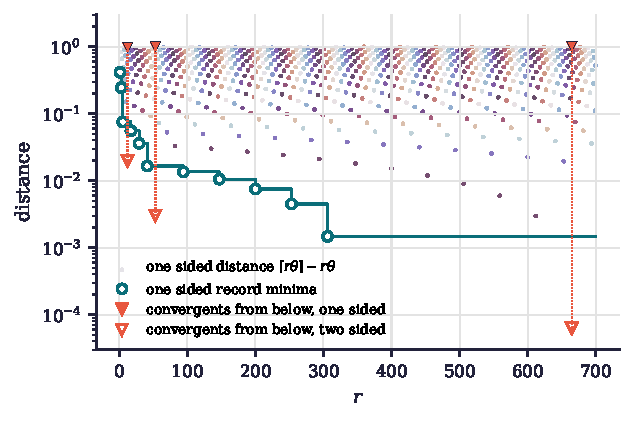
\includegraphics[width=\textwidth]{figures/ch8_onesided.pdf}
\caption{The one sided distance $\delta(r)=\lceil r\theta\rceil-r\theta$ for
$r\leq700$. Circles mark the record minima, which are the rungs
$1,3,5,17,29,41,94,147,200,253,306$. Triangles mark the convergents from below,
$q_4=12$, $q_6=53$ and $q_8=665$: filled at their one sided distance, which is
close to $1$, and open at their two sided distance $\|q\theta\|$, which is
small.}
\label{fig:ch8:onesided}
\end{figure}

\begin{figure}[ht]
\centering
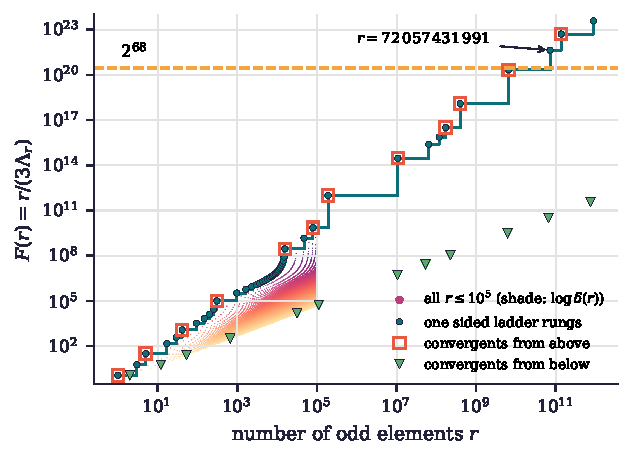
\includegraphics[width=\textwidth]{figures/ch8_records.pdf}
\caption{The bound $F(r)=r/(3\Lambda_r)$ on the least element of a cycle with $r$ odd elements. Shaded by $\log\delta(r)$: all $r\leq10^5$. Staircase: the rungs of the one sided ladder up to $10^{12}$, joined as a running maximum. Squares and triangles: convergent denominators from above and below. The dashed line is the verified range $2^{68}$; the first rung above it is $r=72\,057\,431\,991$.}
\label{fig:ch8:records}
\end{figure}

\section{The mediant lemma}\label{sec:ch8:mediant}

We now show that the rungs are not merely where the records happen to lie in
a finite search, but where they must lie. The argument is a single
observation about the additivity of $\delta$.

\begin{lemma}[Mediant lemma]\label{lem:ch8:mediant}
Let $1\leq r'<r$ with $\delta(r')<\delta(r)$, and put $d=r-r'$. Then
\begin{equation}\label{eq:ch8:additive}
  \delta(r)=\delta(r')+\delta(d).
\end{equation}
Consequently $\delta(r)/r$ is the mediant of $\delta(r')/r'$ and
$\delta(d)/d$, and
\begin{equation}\label{eq:ch8:mediantineq}
  \frac{\delta(r)}{r}\geq\min\Bigl(\frac{\delta(r')}{r'},\
  \frac{\delta(d)}{d}\Bigr).
\end{equation}
\end{lemma}

\begin{proof}
For every $x\geq1$, $\delta(x)=\lceil x\theta\rceil-x\theta$ is congruent to
$-x\theta$ modulo $1$ and lies in $(0,1)$; since $x\theta\notin\Z$, it is
the unique number in $[0,1)$ with that property. The number
$\delta(r)-\delta(r')$ is congruent to $-(r-r')\theta=-d\theta$ modulo $1$, and
by hypothesis it lies in $(0,1)$, because both terms lie in $(0,1)$ and the
first is larger. By uniqueness it equals $\delta(d)$. For the inequality,
$\delta(r)/r=(\delta(r')+\delta(d))/(r'+d)$ is a weighted average of
$\delta(r')/r'$ and $\delta(d)/d$, with weights $r'/r$ and $d/r$, and is
therefore at least the smaller of the two.
\end{proof}

The content of \eqref{eq:ch8:additive} is that there is no wrap around: the
congruence $\delta(r)\equiv\delta(r')+\delta(d)$ modulo $1$ always holds, and
the hypothesis $\delta(r')<\delta(r)$ upgrades it to an equality. We now draw
two consequences.

\begin{corollary}\label{cor:ch8:firstfeasible}
Let $\varepsilon>0$ and suppose some $r\geq1$ satisfies
$\delta(r)<r\varepsilon$. Then the smallest such $r$ is a $\delta$ record.
\end{corollary}

\begin{proof}
Let $r_*$ be the smallest $r$ with $\delta(r)<r\varepsilon$, and suppose it is
not a $\delta$ record. Then there is $r'<r_*$ with $\delta(r')\leq\delta(r_*)$.
Equality is impossible, since it would make $(r_*-r')\theta$ an integer; so
$\delta(r')<\delta(r_*)$. Put $d=r_*-r'$, so $1\leq d<r_*$. By minimality of
$r_*$, both $\delta(r')\geq r'\varepsilon$ and $\delta(d)\geq d\varepsilon$.
By \eqref{eq:ch8:mediantineq}, $\delta(r_*)/r_*\geq\varepsilon$, a
contradiction.
\end{proof}

\begin{corollary}\label{cor:ch8:recordsrecords}
If $r$ is a strict record of $r\mapsto r/\delta(r)$, meaning
$r/\delta(r)>r'/\delta(r')$ for every $1\leq r'<r$, then $r$ is a $\delta$
record.
\end{corollary}

\begin{proof}
If not, there is $r'<r$ with $\delta(r')<\delta(r)$ (equality being impossible
as before). With $d=r-r'<r$, \eqref{eq:ch8:mediantineq} gives
$r/\delta(r)\leq\max(r'/\delta(r'),d/\delta(d))$, contradicting strictness.
\end{proof}

Since $F(r)=r/(3\delta(r)\log2)$ is a constant multiple of $r/\delta(r)$,
\cref{cor:ch8:recordsrecords} combined with \cref{thm:ch8:onesided} locates
the records of $F$ exactly.

\begin{proposition}[Where the records are]\label{prop:records}
Every $r$ at which $r\mapsto F(r)=r/(3\Lambda_r)$ attains a strict record is a
rung of the semiconvergent\index{convergent}\index{semiconvergent} ladder approximating $\theta$ from above, that is,
$r=q_{k-1}+jq_k$ with $k\geq0$ even and $1\leq j\leq a_{k+1}$. Moreover, for
every verified range\index{verification range} $X$, the smallest $r$ that is not excluded in the sense
of \cref{def:ch8:excl} is such a rung.
\end{proposition}

\begin{proof}
The first statement is \cref{cor:ch8:recordsrecords} combined with
\cref{thm:ch8:onesided}. The second is \cref{cor:ch8:firstfeasible} with
$\varepsilon=1/(3X\log2)$, followed by \cref{thm:ch8:onesided}. (Such an $r$
exists: by \cref{lem:ch8:basic}(iv), at the convergents from above
$\delta(q_k)=p_k-q_k\theta<1/q_{k+1}$, which is eventually below
$q_k\varepsilon$.)
\end{proof}

The converse holds as well, so the strict records of $F$ are exactly the rungs, as the classical theorem~\cite[Theorem~4.5(ii)]{hancl2019} also says. Along the rungs $r$ increases while $\delta$ decreases, by \cref{thm:ch8:onesided}, so $F$ increases; and for any $r'$ the first point at which $F$ attains its maximum over $[1,r']$ is a strict record, hence a rung $u'\leq r'$, so every rung $u>r'$ has $F(u)>F(u')\geq F(r')$.
For $\lt$ every rung
up to $72\,057\,431\,991$ is accordingly a record of $F$ (the values in
\cref{tab:ch8:ladder} increase), and the exact scan to $3\times10^6$ found
the records of $F$ and the $\delta$ records to coincide there. The cycle bound
below does not need the converse.

\begin{remark}[Ties, and a warning about arithmetic]\label{rem:ch8:ties}
Multiples of a rung produce exact ties. If $t\,\delta(q)<1$ for an integer $t\geq2$ then
$\delta(tq)=t\,\delta(q)$, since $tq\theta=t\lceil q\theta\rceil-t\delta(q)$,
so $F(tq)=F(q)$ and the multiple ties with its generator rather than beating
it; by \cref{cor:ch8:recordsrecords} it cannot be a strict record.
Halbeisen\index{Halbeisen, L.} and Hungerb\"uhler\index{Hungerbuhler, N.@Hungerb\"uhler, N.}~\cite[\S4.4]{halbeisen1997} observe these ties for Eliahou's criterion, at multiples of a convergent denominator. In floating
point arithmetic such ties break at random. With $\Lambda_r$ evaluated in
double precision as $s\log2-r\log3$, $s=\lfloor r\theta\rfloor+1$, a scan of
$r\leq10^6$ reports $918=3\cdot306$, $46\,803=3\cdot15\,601$ and
$952\,685=5\cdot190\,537$ as new records (script \texttt{ch08\_ties.py});
evaluated instead as $(\lceil r\theta\rceil-r\theta)\log2$, the same scan
happens to report no spurious records, the ties breaking the other way or not
at all.
At $150$ digits the differences $\delta(tq)-t\delta(q)$ for $46\,803$, $571\,611=3\cdot190\,537$ and $952\,685$ come out as $-2.5\times10^{-147}$, $0$ and $0$, but the spurious records do not disappear: a tie is an exact equality between irrational numbers, so rounding decides it at every precision, and the same scan at $150$ digits reports $15=3\cdot5$ and $571\,611$ as new records in the first form, and $46\,803$ and $571\,611$ in the second.
The cure is exact arithmetic: $F(r)>F(r')$ if and only if $r\lceil r'\theta\rceil>r'\lceil r\theta\rceil$, a comparison of integers once the ceilings are known, and a scan of $r\leq10^6$ in this form finds exactly the rungs as its strict records.
This is one more reason to prefer an argument that locates the records over
a search that merely finds them.
\end{remark}

\section{The cycle length bound}\label{sec:ch8:bound}

\Cref{prop:records} turns the search for the sharp bound into a short
computation over the rungs. For $\lt$ there are only $44$ rungs up to
$72\,057\,431\,991$, and \cref{tab:ch8:ladder} lists the last eleven of them
with the value of $F$ at each.

\begin{table}[ht]
\centering
\caption{The upper ladder rungs from $q_9$ to the first rung exceeding
$2^{68}$, with $s=\lceil r\theta\rceil$ and $F(r)=r/(3\Lambda_r)$, computed
at $150$ digits. The decomposition column writes each rung as a convergent denominator or as
$q_{k-1}+jq_k$.}
\label{tab:ch8:ladder}
\small
\begin{tabular}{@{}rrrl@{}}
\toprule
$r$ & $s$ & $F(r)$ & rung \\
\midrule
$15\,601$ & $24\,727$ & $2.86\times10^{8}$ & $q_9$ \\
$47\,468$ & $75\,235$ & $1.45\times10^{9}$ & $q_9+q_{10}$ \\
$79\,335$ & $125\,743$ & $7.22\times10^{9}$ & $q_{11}$ \\
$190\,537$ & $301\,994$ & $9.85\times10^{11}$ & $q_{13}=q_{11}+q_{12}$ \\
$10\,781\,274$ & $17\,087\,915$ & $2.94\times10^{14}$ & $q_{15}=q_{13}+q_{14}$ \\
$64\,497\,107$ & $102\,225\,496$ & $2.46\times10^{15}$ & $q_{15}+q_{16}$ \\
$118\,212\,940$ & $187\,363\,077$ & $7.49\times10^{15}$ & $q_{15}+2q_{16}$ \\
$171\,928\,773$ & $272\,500\,658$ & $3.20\times10^{16}$ & $q_{17}$ \\
$397\,573\,379$ & $630\,138\,897$ & $1.25\times10^{18}$ & $q_{19}=q_{17}+q_{18}$ \\
$6\,586\,818\,670$ & $10\,439\,860\,591$ & $2.17\times10^{20}$ & $q_{21}=q_{19}+q_{20}$ \\
$72\,057\,431\,991$ & $114\,208\,327\,604$ & $4.36\times10^{21}$ & $q_{21}+q_{22}$ \\
\bottomrule
\end{tabular}
\end{table}

\begin{theorem}[Cycle length bound]\label{thm:cycles}
Let $X$ be a verified range\index{verification range} in the sense of \cref{def:ch8:excl}.
\begin{enumerate}[label=(\roman*),leftmargin=2em]
\item \emph{Block form.} If $B_j\leq X$ for $j=0,1,\dots,K$, then every
  nontrivial cycle has $r\geq q_{K+1}$ odd elements.
\item \emph{Sharp form.} Every nontrivial cycle has $r\geq r_*(X)$ odd
  elements, where $r_*(X)$ is the smallest rung $u$ of the upper ladder with
  $F(u)>X$.
\end{enumerate}
With $X=2^{68}$, verified by Ba\v{r}ina\index{Barina, D.@Ba\v{r}ina, D.}~\cite{barina2021}, part (i) gives
\[
  r\geq q_{21}=6\,586\,818\,670,
\]
and part (ii) gives
\[
  r\geq72\,057\,431\,991,\qquad s\geq114\,208\,327\,604 .
\]
Thus a nontrivial cycle has at least $7.2\times10^{10}$ steps of $S$, at least
$1.14\times10^{11}$ steps of $T$, and at least $1.86\times10^{11}$ steps of
$T_0$.
\end{theorem}

\begin{proof}
By \cref{cor:ch8:excl} the number $r$ of odd elements of a nontrivial cycle is
not excluded, so $F(r)>X$.

(i) If $1\leq r<q_{K+1}$, then $q_j\leq r<q_{j+1}$ for some $0\leq j\leq K$
(recall $q_0=1$), and \cref{lem:block} gives $F(r)<B_j\leq X$, so $r$ is
excluded. With $X=2^{68}$, \cref{tab:cycles} and the values for $k\leq7$ in
its caption show $B_j\leq B_{20}=2.29\times10^{19}<2^{68}$ for all $j\leq20$,
so $K=20$ is admissible and $r\geq q_{21}$.

(ii) By \cref{prop:records}, the smallest nonexcluded $r$ is an upper ladder
rung $u$, and by definition of exclusion it is the smallest rung with
$F(u)>X$. So every $r<r_*(X)$ is excluded. With $X=2^{68}$, the $44$ rungs up
to $72\,057\,431\,991$ were evaluated at $150$ digits (script
\texttt{ch08\_bounds.py}); all before the last have $F(u)\leq
2.1689\times10^{20}<2^{68}=2.9515\times10^{20}$, the maximum being attained at
$u=q_{21}$, while $F(72\,057\,431\,991)=4.3585\times10^{21}>2^{68}$. Hence
$r_*(2^{68})=72\,057\,431\,991$. For the number of halvings, $s>r\theta\geq
r_*\theta$ and $s$ is an integer, so $s\geq\lceil r_*\theta\rceil=
114\,208\,327\,604$. The step counts follow from
\cref{rem:ch8:bookkeeping}: $r$ steps of $S$, $s$ of $T$ and $r+s\geq
186\,265\,759\,595$ of $T_0$.
\end{proof}

The first part uses only the property of best
approximation, and the second part uses the one sided theorem and the mediant lemma\index{mediant lemma}, and the numerical
evaluation involves margins that are enormous compared with the precision
used: the closest call is the ratio $2^{68}/F(q_{21})=1.36$, and the values of
$\delta$ involved are of order $10^{-11}$, computed with errors below
$10^{-130}$. The factor of about eleven between the two parts measures what
the block bound gives away by covering a whole interval with a single worst
case.

With the verification range $2^{71}$ of Ba\v{r}ina\index{Barina, D.@Ba\v{r}ina, D.}~\cite{barina2025}, part (i) improves to $r\geq q_{22}=65\,470\,613\,321$, since $B_{21}=2.16\times10^{21}<2^{71}=2.36\times10^{21}$, while part (ii) is unchanged, since $F(72\,057\,431\,991)=4.36\times10^{21}>2^{71}$.

\subsection{Exact versus crude}

There is an intermediate argument, which uses the $\delta$ records but not
the mediant lemma\index{mediant lemma}, and it can be much weaker. Let
$q_1'<q_2'<\cdots$ be the $\delta$ records. If a cycle has $r$ odd elements
and $q_j'$ is the largest record not exceeding $r$, then
$\delta(r)\geq\delta(q_j')$ by the definition of a record, and
$\delta(r)<r\varepsilon$ by \cref{cor:ch8:excl}, so $r>\delta(q_j')/\varepsilon$
and $r\geq q_j'$. Minimizing over the unknown $j$,
\begin{equation}\label{eq:ch8:crude}
  r\geq\min_j\max\Bigl(q_j',\ \frac{\delta(q_j')}{\varepsilon}\Bigr).
\end{equation}
The same bound appears in our unpublished note on AlphaProof
Nexus~\cite{polsonsokolov2026nexus}. It is valid, but loose. The reason is that
it uses the single value $\delta(q_j')$ as a lower bound for $\delta$ on the
whole block $[q_j',q_{j+1}')$, so it cannot exclude any $r$ in that block
beyond $\delta(q_j')/\varepsilon$, even though $\delta(r)$ there is in fact
much larger. The mediant lemma shows that nothing inside a block needs to be
checked at all: only the rungs matter, and at each rung one compares the exact
$\delta$ with $r\varepsilon$. \Cref{tab:ch8:crude} compares the two for
several verification ranges\index{verification range} (script \texttt{ch08\_crude.py}, at $80$ digits).

\begin{table}[ht]
\centering
\caption{Lower bounds on the number $r$ of odd elements of a nontrivial cycle,
for several verification ranges $X$: the exact first nonexcluded $r$ of
\cref{thm:cycles}(ii), with the corresponding $s=\lceil r\theta\rceil$, and
the crude bound \eqref{eq:ch8:crude}. The ranges up to $2^{71}$ are
verified~\cite{barina2021,barina2025}; the row $2^{72}$ shows what the method would give.}
\label{tab:ch8:crude}
\small
\begin{tabular}{@{}lrrr@{}}
\toprule
$X$ & exact $r_*(X)$ & $s$ & crude bound \\
\midrule
$2^{40}$ & $10\,781\,274$ & $17\,087\,915$ & $212\,781$ \\
$2^{60}$ & $397\,573\,379$ & $630\,138\,897$ & $397\,573\,379$ \\
$2^{68}$ & $72\,057\,431\,991$ & $114\,208\,327\,604$ & $8\,963\,457\,697$ \\
$2^{71}$ & $72\,057\,431\,991$ & $114\,208\,327\,604$ & $71\,707\,661\,575$ \\
$2^{72}$ & $137\,528\,045\,312$ & $217\,976\,794\,617$ & $78\,073\,328\,038$ \\
\bottomrule
\end{tabular}
\end{table}

At $2^{40}$ the crude bound is fifty times weaker: it is determined by the
record $q_{13}=190\,537$, with $\delta(q_{13})/\varepsilon=212\,780.2$, whereas
the next rung that is actually feasible is $q_{15}=10\,781\,274$. At $2^{68}$
the crude bound is determined by $q_{21}$, with
$\delta(q_{21})/\varepsilon=8\,963\,457\,696.8$, and it is eight times weaker
than the exact value. At $2^{60}$ the two coincide: the record $q_{19}=397\,573\,379$ is
itself feasible, and the preceding record $q_{17}$ has
$\delta(q_{17})/\varepsilon\approx6.2\times10^{9}$, which already exceeds
$q_{19}$, so the minimum in \eqref{eq:ch8:crude} is attained at $q_{19}$
with value $q_{19}$.

The table also shows how slowly the exact bound responds to verification.
Moving from $2^{68}$ to $2^{71}$, the step taken by Ba\v{r}ina\index{Barina, D.@Ba\v{r}ina, D.}~\cite{barina2025}, gives the exact bound no improvement whatever, because the
rung $r=72\,057\,431\,991$ has $F(r)=4.3585\times10^{21}=2^{71.884}$: any
verified range below about $2^{71.9}$ leaves that rung feasible. For the sharp form of \cref{thm:cycles}, a
verification past that point, for instance to $2^{72}$, would move the bound
to the next rung, $r\geq137\,528\,045\,312=q_{23}$, and further progress would
require passing $F(q_{23})=5.10\times10^{22}$. The bound $r\geq137\,528\,045\,312$ itself already holds unconditionally: it is the current record, which follows from Hercher's sharper accounting of the cycle together with the verification to $2^{71}$ (\cref{rem:attribution}).
The return on computation is
stepwise, in a way dictated entirely by the
continued fraction\index{continued fraction}; over many steps the bound grows roughly like the
square root of the verified range, from $1.08\times10^{7}$ at $2^{40}$ to
$7.2\times10^{10}$ at $2^{68}$.


\subsection{Verification thresholds}\label{sec:ch8:thresholds}

Since $r_*(X)$ is a step function of the verification range\index{verification range}, it is natural to
ask exactly where the steps are. The first rung $u$ not excluded at $X$ changes
precisely when $\log_2X$ crosses $\log_2F(u)$ for the current rung $u$, so the
thresholds are the values $\log_2F(u)$ along the sequence of successive
$r_*$. \Cref{tab:ch8:thresholds} lists them for $60\le\log_2X\le90$ and
\cref{fig:ch8:thresholds} draws the staircase (script
\texttt{ch08\_profile.py}, at $700$ digits).

\begin{table}[ht]
\centering\small
\caption{The sharp bound $r_*(X)$ as a function of the verification range.
Each row gives the rung $r_*$, the corresponding $s=\lceil r_*\theta\rceil$
and the interval of $\log_2X$ on which it is the bound.}
\label{tab:ch8:thresholds}
\begin{tabular}{@{}rrc@{}}
\toprule
$r_*$ & $s$ & range of $\log_2X$ \\
\midrule
$397\,573\,379$ & $630\,138\,897$ & $[54.830,\ 60.119)$ \\
$6\,586\,818\,670$ & $10\,439\,860\,591$ & $[60.119,\ 67.556)$ \\
$72\,057\,431\,991$ & $114\,208\,327\,604$ & $[67.556,\ 71.884)$ \\
$137\,528\,045\,312$ & $217\,976\,794\,617$ & $[71.884,\ 75.433)$ \\
$890\,638\,885\,193$ & $1\,411\,629\,234\,715$ & $[75.433,\ 78.333)$ \\
$1\,643\,749\,725\,074$ & $2\,605\,281\,674\,813$ & $[78.333,\ 79.456)$ \\
$2\,396\,860\,564\,955$ & $3\,798\,934\,114\,911$ & $[79.456,\ 80.287)$ \\
$5\,409\,303\,924\,479$ & $8\,573\,543\,875\,303$ & $[82.796,\ 84.500)$ \\
$11\,571\,718\,688\,839$ & $18\,340\,740\,190\,704$ & $[84.500,\ 87.951)$ \\
$64\,021\,008\,208\,555$ & $101\,470\,897\,268\,921$ & $[87.951,\ 90.590)$ \\
\bottomrule
\end{tabular}
\end{table}

Three features stand out. The range $2^{68}$ of \cref{thm:cycles} sits just above a
threshold, at $67.556$, which is why it yields the rung $72\,057\,431\,991$
rather than $6\,586\,818\,670$. The current range $2^{71}$~\cite{barina2025} lies in the same step, and so does the range $1536\cdot2^{60}=2^{70.585}$ at which Hercher\index{Hercher, C.}~\cite[Corollary~29]{hercher2023} obtains $r\geq1.375\times10^{11}$, now the record;
so the difference between our bound and that
record comes entirely from his sharper accounting of the
cycle, not from a larger range. And the steps between $2^{78}$ and $2^{83}$
are close together, because the partial quotient $a_{25}=7$ produces a ladder of seven nearby rungs $q_{23}+jq_{24}=137\,528\,045\,312+j\cdot753\,110\,839\,881$, $1\leq j\leq7$, of which the table shows the
first three and the last; the intermediate rungs occupy $[80.287,\ 82.796)$.

\begin{figure}[ht]
\centering
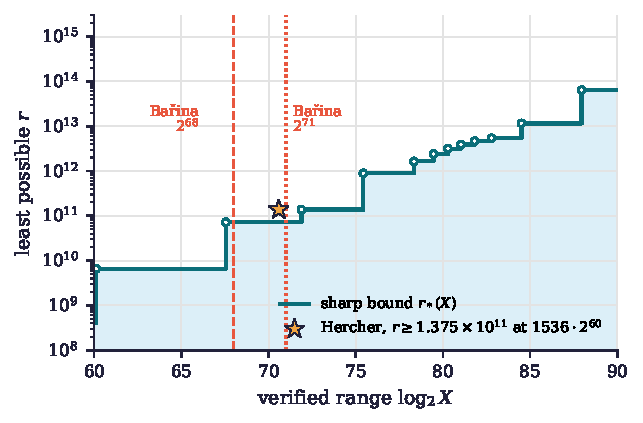
\includegraphics[width=\textwidth]{figures/ch8_thresholds.pdf}
\caption{The sharp bound $r_*(X)$ against the verification range $\log_2X$.
Every step is a rung of the one sided ladder of $\lt$. The dashed line marks
the range $2^{68}$ of Ba\v{r}ina~\cite{barina2021} and the dotted line his current range $2^{71}$~\cite{barina2025}, which lies in the same step. The star is the bound $r\geq1.375\times10^{11}$ that Hercher's sharper accounting of the cycle gives at
$1536\cdot2^{60}$; conditional when it was published, it is the current record since the verification to $2^{71}$.}
\label{fig:ch8:thresholds}
\end{figure}

\subsection{The literature}

\begin{remark}[Attribution]\label{rem:attribution}
The method of this section is not new, and we claim no priority for any
numerical bound. It goes back to Crandall\index{Crandall, R. E.}~\cite{crandall1978}, whose criterion is in substance the block bound of \cref{lem:block}, and to Eliahou~\cite{eliahou1993}. Steiner\index{Steiner, R. P.}~\cite{steiner1977} showed in 1977 that there is no
nontrivial cycle consisting of a single ascending run followed by a single
descending run (a $1$ cycle), using the continued fraction\index{continued fraction} of $\lt$ together
with Baker\index{Baker, A.}'s theory\index{Baker method} of linear forms in logarithms. Eliahou\index{Eliahou, S.}~\cite{eliahou1993}
combined the continued fraction of $\theta$ with verification to $2^{40}$ and
showed in 1993 that a nontrivial cycle has at least $17\,087\,915$ elements
under $T$; our method reproduces this figure exactly, as the value of $s$ at
$r_*(2^{40})=10\,781\,274$ in \cref{tab:ch8:crude}, which we regard as a
check on the implementation. The figure $q_{21}=6\,586\,818\,670$ of \cref{thm:cycles}(i) is also in the literature: Lagarias\index{Lagarias, J. C.}'s overview~\cite[\S6.1, item~(W2)]{lagarias2010overview} reports it from Eliahou's criterion with the smaller verification range $20\cdot2^{58}\approx5.76\times10^{18}$ of item~(W1). The bound $r\geq72\,057\,431\,991$ of \cref{thm:cycles}(ii) coincides with the record $r>7.2\times10^{10}$ that Hercher\index{Hercher, C.}~\cite{hercher2023} credits to Hercher and Puchert\index{Puchert, S.}~\cite{hercher2018,puchert2018}; with the verification range $87\cdot2^{60}$, Hercher~\cite{hercher2018} had shown that a nontrivial cycle has at least $p_{21}+q_{21}=17\,026\,679\,261$ elements under $T_0$.
Simons\index{Simons, J.} and de Weger\index{de Weger, B.}~\cite{simons2005} extended
Steiner's approach to $m$ cycles, cycles with $m$ ascending runs, ruling them
out for $m\leq68$ by combining continued fractions and lattice reduction with an explicit lower bound for $s\log2-r\log3$ derived from Rhin\index{Rhin, G.}'s Pad\'e approximation measure~\cite{rhin1987}, and
Hercher\index{Hercher, C.}~\cite[Theorem~23]{hercher2023} carried this to $m\leq91$. Hercher~\cite[Corollary~29]{hercher2023} also showed, by a sharper accounting of the
cycle structure than the crude inequality $\log(1+1/(3x_i))\leq1/(3M)$ used
in \cref{lem:cycleid}, that verification\index{verification range} up to $3\cdot2^{69}=1536\cdot2^{60}$ would give $r\geq1.375\times10^{11}$; with the crude inequality one needs $3781\cdot2^{60}$, the value $4.36\times10^{21}$ of $F$ at $r=72\,057\,431\,991$~\cite[Remark~28]{hercher2023}. Ba\v{r}ina\index{Barina, D.@Ba\v{r}ina, D.}~\cite{barina2025} has since verified the conjecture up to $2^{71}>3\cdot2^{69}$, so this bound now holds unconditionally and is the current record: every nontrivial cycle has $r\geq137\,528\,045\,312=q_{23}$ odd elements, and at least $p_{23}+q_{23}=355\,504\,839\,929$ elements under $T_0$, as Ba\v{r}ina notes~\cite[\S6]{barina2025}.
The record structure itself is classical: the first
nonexcluded $r$ is the least denominator of a fraction $s/r$ in the interval
$(\theta,\theta+\varepsilon)$, and the least denominator fraction in an interval
is read off the continued fraction expansion, a lemma Hercher states and uses
(his Lemma 22) and which underlies Eliahou's computation; in the form of \cref{thm:ch8:onesided} and \cref{prop:records} it is the description of the best one sided approximations stated and proved in~\cite[Theorem~4.5(ii)]{hancl2019}. The mediant lemma\index{mediant lemma}
(\cref{lem:ch8:mediant}) reduces the question to the $\delta$ records in two lines, and \cref{thm:ch8:onesided} identifies those with the rungs;
together they keep the certificate\index{certificate} of \cref{sec:ch8:certificate} short. Halbeisen\index{Halbeisen, L.} and Hungerb\"uhler\index{Hungerbuhler, N.@Hungerb\"uhler, N.}~\cite{halbeisen1997} go further in another direction: they replace the crude inequality by the optimal criterion, which is attained by the balanced parity word, and they observe both the harmlessness of the convergents from the wrong side (\cref{rem:ch8:false}) and the exact ties at multiples (\cref{rem:ch8:ties}). What we add
is that certificate and the analysis of \cref{sec:ch8:limits}, which shows exactly what Diophantine\index{Diophantine approximation}
information cannot do (a point that Halbeisen and Hungerb\"uhler~\cite[\S5]{halbeisen1997} make in another form: rational cycles satisfy the same inequalities, and their least elements grow with the length) and what arithmetic information would suffice.
\end{remark}

\begin{remark}[Comparison with Baker's method]\label{rem:ch8:baker}
Baker's theory gives lower bounds for linear forms in logarithms of algebraic
numbers, and for two logarithms the explicit estimates of Laurent\index{Laurent, M.}, Mignotte\index{Mignotte, M.}
and Nesterenko\index{Nesterenko, Yu.}~\cite[Corollary~2]{laurent1995} give, for the form
$\Lambda=s\log2-r\log3$, a bound of the shape $\log\Lambda\geq-C(\log r)^2$
with an explicit absolute constant $C$; precisely, $\log\Lambda\geq-24.34\,\log3\,\bigl(\max\{\log b'+0.14,\,21\}\bigr)^2$ with $b'=r+s/\log3\approx2.44\,r$.
For $r\leq4.6\times10^8$ the maximum is $21$ and the bound is $-24.34\cdot\log3\cdot441\approx-11\,792$, so it gives only $\Lambda\geq e^{-11800}$ there, and $\Lambda\geq e^{-11900}$ for $r\leq5\times10^8$: a bound on
$M$ that is astronomically larger than anything verification can reach,
whereas the actual values of $\Lambda_r$ near $r=10^5$, from
\cref{tab:ch8:conv}, are of order $10^{-6}$. The reason is structural. Baker's
theorem bounds $\Lambda$ uniformly in $r$, with no knowledge of which $r$ are
dangerous; here we enumerate the dangerous $r$, so the exact value of
$\Lambda_r$ is available. Transcendence methods become indispensable only
when a bound valid for all $r$ simultaneously is wanted, as for the $m$ cycle
results of Steiner, Simons and de Weger, and Hercher, where $r$ is unbounded.
\end{remark}

\section{What Diophantine approximation cannot do}\label{sec:ch8:limits}

One might believe that the cycle half of the conjecture is, at bottom,
a question about how well $\lt$ can be approximated by rationals, and that a
sufficiently strong effective irrationality measure\index{irrationality measure} for $\lt$ would settle it.
This section shows that the belief is false, quantifies what such a measure
would give, and identifies the missing ingredient.

\begin{remark}[What an irrationality measure gives]\label{rem:irrmeasure}
Suppose $\nu$ is an effective irrationality measure for $\lt$ with constant
$c$, meaning that $|\lt-s/r|\geq c\,r^{-\nu}$ for all integers $s$ and
$r\geq1$. Then $\delta(r)=s-r\theta=r(s/r-\theta)\geq c\,r^{1-\nu}$ with
$s=\lceil r\theta\rceil$, and \eqref{eq:ch8:maxM} becomes
\begin{equation}\label{eq:ch8:irrbound}
  M<F(r)\leq\frac{r^{\nu}}{3c\log2}.
\end{equation}
Since $\nu\geq2$ for every irrational number (\cref{lem:ch8:basic}(iv)), the
right side grows at least like $r^2$. Combined with $M>X$, the bound excludes
precisely the $r$ with $r^{\nu}<3cX\log2$, a finite range, and nothing beyond
it. In particular no irrationality measure, however good, bounds $M$ uniformly in $r$.
\end{remark}

The finite range is not a weakness of irrationality measures in particular.
It is forced by the structure of the problem.

\begin{proposition}[Diophantine insufficiency]\label{prop:ch8:insufficient}
For every $X\geq1$ there are infinitely many $r\geq1$ with
\[
  0<\delta(r)<\frac{r}{3X\log2},
\]
that is, infinitely many $r$ that are not excluded at verification range\index{verification range} $X$.
\end{proposition}

\begin{proof}
By \cref{thm:ch8:onesided} the one sided records $u_1<u_2<\cdots$ form an
infinite sequence along which $\delta(u_i)$ decreases strictly. Moreover
$\delta(u_i)\to0$: the convergents\index{convergent} $p_k/q_k$ with $k$ odd lie above $\theta$,
so $\lceil q_k\theta\rceil=p_k$ and $\delta(q_k)=p_k-q_k\theta<1/q_{k+1}$ by
\cref{lem:ch8:basic}(iv), and these $q_k$ are among the records. Put
$\varepsilon=1/(3X\log2)$. Once $\delta(u_i)<\varepsilon$, which holds for all
large $i$, we have $\delta(u_i)<\varepsilon\le u_i\varepsilon$, so $u_i$ is
not excluded.
\end{proof}

In words: the inequality \eqref{eq:ch8:maxM}, a verified range and any information about the number $\lt$ alone cannot together exclude all nontrivial cycles.

How large is the gap in practice? The best conceivable constant for $\nu=2$
consistent with the rungs computed so far is $c_2=\min_u u\,\delta(u)
=0.01773$, attained at $u=190\,537$ (the rung before the partial quotient
$55$), and the corresponding exclusion is $r<(3c_2X\log2)^{1/2}$.
\Cref{tab:ch8:insufficient} compares this with the exact $r_*(X)$. Even this
idealized measure, far better than any effective measure known (the explicit bound of Rhin~\cite{rhin1987}, in the form used by Simons and de Weger~\cite[Lemma~12]{simons2005}, corresponds to $\nu\approx14.3$), is beaten by
the ladder computation by factors from about two to more than fifty, because the ladder
uses the exact value of $\delta$ at each dangerous $r$ while the measure uses
a worst case. With exponents $\nu\geq3$ the best conceivable constant is
$c_\nu=\log_2(4/3)=0.4150$, attained at $r=1$, and at $X=2^{68}$ it excludes
only $r<6.3\times10^6$ for $\nu=3$ and $r<1.3\times10^5$ for $\nu=4$.

\begin{table}[ht]
\centering\small
\caption{Exclusion by an idealized measure with $\nu=2$ and $c_2=0.01773$
versus the exact ladder bound.}
\label{tab:ch8:insufficient}
\begin{tabular}{@{}lrrr@{}}
\toprule
$X$ & measure excludes $r<$ & exact $r_*(X)$ & ratio \\
\midrule
$2^{40}$ & $2.01\times10^{5}$ & $1.08\times10^{7}$ & $53.5$ \\
$2^{60}$ & $2.06\times10^{8}$ & $3.98\times10^{8}$ & $1.93$ \\
$2^{68}$ & $3.30\times10^{9}$ & $7.21\times10^{10}$ & $21.8$ \\
$2^{72}$ & $1.32\times10^{10}$ & $1.38\times10^{11}$ & $10.4$ \\
$2^{80}$ & $2.11\times10^{11}$ & $2.40\times10^{12}$ & $11.4$ \\
\bottomrule
\end{tabular}
\end{table}

\Cref{fig:ch8:irrprofile} shows the empirical irrationality profile of $\lt$:
for each convergent the exponent $\nu_k=-\log|\theta-p_k/q_k|/\log q_k$,
together with the next partial quotient. The exponents settle near $2$ (their
mean over $50\le k\le198$ is $2.010$), with excursions exactly where a large
partial quotient follows; the largest partial quotients among the first $199$
are $55$ (twice), $49$, $37$ and $33$. This is what one sees for a typical real
number, and it says nothing provable about $\lt$. In particular the profile
gives no evidence either way on whether the partial quotients of $\lt$ are
bounded; and by \cref{prop:ch8:insufficient}, even bounded partial quotients
would not finish the cycle half.

\begin{figure}[ht]
\centering
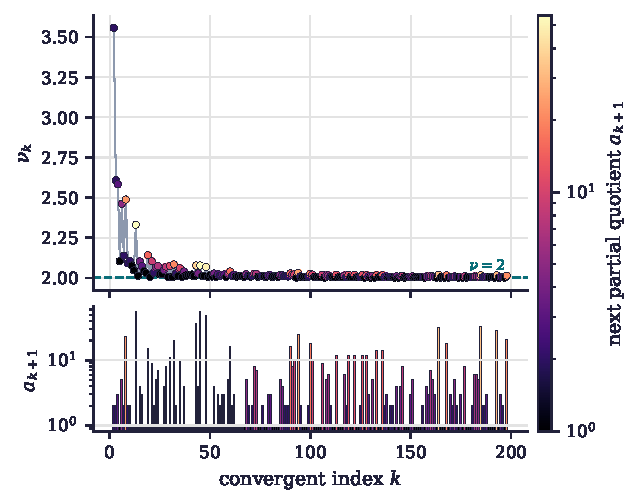
\includegraphics[width=\textwidth]{figures/ch8_irrprofile.pdf}
\caption{Empirical irrationality profile of $\lt$. Top: the exponent $\nu_k$
of the $k$th convergent, coloured by the next partial quotient. Bottom: the
partial quotients $a_{k+1}$ on a logarithmic scale. Large partial quotients
produce the visible excursions above $\nu=2$.}
\label{fig:ch8:irrprofile}
\end{figure}

\subsection{The window lemma}

What, then, is missing? The inequality \eqref{eq:ch8:maxM} is an
\emph{upper} bound on the least element of a cycle. The affine identity of
\cref{chap:parity} gives a matching \emph{lower} bound, and the two together
confine the least element to a window whose width is the real measure of our
ignorance.
In the rest of this section we write $m=r$ for the number of odd steps and $k=s$ for the number of steps of $T$, as in \cref{chap:parity}, so that $k$ is no longer a continued fraction index.

\begin{lemma}[Window lemma]\label{lem:ch8:window}
Let $x_1,\dots,x_r$ be the odd elements of a cycle of the accelerated map\index{accelerated map} $T$
with $r=m$ odd steps and $k=s$ steps in all, and put
$\Lambda=k\log2-m\log3>0$. Then every element $x$ of the cycle (odd or even)
satisfies
\begin{equation}\label{eq:ch8:window}
  \frac{3^m-2^m}{2^k-3^m}\;\le\;x,
  \qquad\text{and}\qquad
  M=\min_i x_i\;<\;\frac{m}{3\Lambda}\;\le\;F(m),
\end{equation}
where $(3^m-2^m)/(2^k-3^m)=(1-(2/3)^m)/(e^{\Lambda}-1)$, and $m/(3\Lambda)=F(m)$ exactly when $k=\lceil m\theta\rceil$. In particular the least
element lies in the window
$\bigl[(1-(2/3)^m)/(e^{\Lambda}-1),\ m/(3\Lambda)\bigr)$, whose endpoints have
ratio $\frac m3\cdot\frac{e^\Lambda-1}{\Lambda}(1-(2/3)^m)^{-1}$, which is
$\frac m3(1+o(1))$ as $\Lambda\to0$ and $m\to\infty$.
\end{lemma}

\begin{proof}
Let $x$ be any element of the cycle. Applying \eqref{eq:ch2:affine} to the
$k$ steps that return $x$ to itself gives $2^kx=3^mx+c_k(x)$, so
$x=c_k(x)/(2^k-3^m)$, the denominator being positive because $\Lambda>0$. By
the recursion \eqref{eq:ch2:crec}, an odd step at time $i$ contributes $2^i$,
multiplied by $3$ once for each later odd step, so
$c_k(x)=\sum_{j=0}^{m-1}3^{m-1-j}2^{i_j}$, where $0\le i_0<i_1<\cdots<i_{m-1}\le
k-1$ are the times of the odd steps. Since $i_j\ge j$, every term is at least
the corresponding term with $i_j=j$, hence
$c_k(x)\ge\sum_{j=0}^{m-1}3^{m-1-j}2^{j}=3^m-2^m$. This gives the lower bound,
and dividing numerator and denominator by $3^m$ gives the second form.
For the upper bound, the proof of \cref{lem:cycleid} with $r=m$ gives $\Lambda<\sum_i1/(3x_i)\le m/(3M)$, since $\log(1+u)<u$; and $\Lambda\ge\Lambda_m=\delta(m)\log2$ by \eqref{eq:ch8:Lambdar}, with equality exactly when $k=\lceil m\theta\rceil$, so $m/(3\Lambda)\le F(m)$.
The ratio of the endpoints is the quotient of the two
expressions, and $(e^\Lambda-1)/\Lambda\to1$, $(2/3)^m\to0$.
\end{proof}

For the trivial cycle, $m=1$ and $k=2$, the window is $[1,\ 1.159)$ and the
cycle sits at its left end. For the hypothetical cycles at the ladder rungs the
window is enormous: at the rung $r_*=72\,057\,431\,991$, with $k$ the
corresponding $s$, the lower end is $1.8\times10^{11}\approx2^{37.4}$ and the
upper end $4.4\times10^{21}=2^{71.9}$, a factor $r/3$ apart as the lemma
predicts (\cref{fig:ch8:window}). The verified range\index{verification range} $2^{68}$ removes the lower
part of the window, and what is left is exactly the gap that the sharp bound
of \cref{thm:cycles} measures.

\begin{corollary}[What arithmetic would suffice]\label{cor:ch8:window}
Suppose that for some function $f$ every nontrivial cycle with $m$ odd steps and $k$ steps in all satisfied the sharpened upper bound $M<m/(3\Lambda f(m))$, where $\Lambda=k\log2-m\log3$ is the value at that cycle.
\begin{enumerate}[label=(\roman*),leftmargin=2em]
\item If $f(m)\ge\frac m3\cdot\frac{e^{\Lambda}-1}{\Lambda}\bigl(1-(2/3)^m\bigr)^{-1}$ for every pair $(m,k)$ with $m\theta<k<2m$, then there are no nontrivial cycles.
\item If $f(m)\ge\frac m3(1+\eta)$ for some $\eta>0$ and all $m\ge m_0$, where $(1+\eta)(1-(2/3)^{m_0})>1$, let $\Lambda_0>0$ solve $(e^{\Lambda_0}-1)/\Lambda_0=(1+\eta)(1-(2/3)^{m_0})$. Then every nontrivial cycle with $m\ge m_0$ odd steps has least element $M<C=1/((1+\eta)\Lambda_0)$, which is about $1/(2\eta)$ when $\eta$ is small and $m_0$ large; so a verified range\index{verification range} $X\ge\max\bigl(C,\max_{m<m_0}F(m)\bigr)$ excludes all nontrivial cycles, with no further use of Diophantine\index{Diophantine approximation} approximation.
\end{enumerate}
\end{corollary}

\begin{proof}
A nontrivial cycle contains no element $1$, so every $x_i\ge3$ and \eqref{eq:ch8:prod} gives $2^k=\prod_i(3+1/x_i)<4^m$; with $\Lambda>0$ this is $m\theta<k<2m$.
(i) The hypothesis puts the upper end $m/(3\Lambda f(m))$ of the sharpened window at or below the lower end $(1-(2/3)^m)/(e^{\Lambda}-1)$ of \eqref{eq:ch8:window}, which is impossible.
(ii) The function $(e^{\Lambda}-1)/\Lambda$ increases from $1$ to $\infty$ on $(0,\infty)$.
For a cycle with $m\ge m_0$ and $\Lambda<\Lambda_0$ it is therefore below $(1+\eta)(1-(2/3)^{m_0})\le\frac{3f(m)}{m}(1-(2/3)^m)$, and the window is empty as in (i).
For a cycle with $m\ge m_0$ and $\Lambda\ge\Lambda_0$ the hypothesis gives $M<m/(3\Lambda_0f(m))\le1/((1+\eta)\Lambda_0)=C$.
For $m<m_0$, \cref{lem:ch8:window} gives $M<F(m)$.
So a nontrivial cycle would have $M<X$, whereas every element of a nontrivial cycle is at least $X$.
\end{proof}

The corollary converts the vague hope that ``the arithmetic of the parity word should help'' into a precise target: an improvement of the upper bound by a factor slightly more than $m/3$. A factor $\frac m3(1+\eta)$ for all large $m$ would confine the least element of every nontrivial cycle with many odd steps below about $1/(2\eta)$, and a finite verification would then exclude all nontrivial cycles.
Raising the lower end by such a factor, or splitting the factor between the two ends, empties the window only when $\Lambda$ is small; the cycles with $\Lambda$ bounded below would still need an upper bound on $M$ that does not grow with $m$.
By contrast, \cref{prop:ch8:insufficient}
shows that no improvement of the Diophantine side alone can work.

\begin{figure}[ht]
\centering
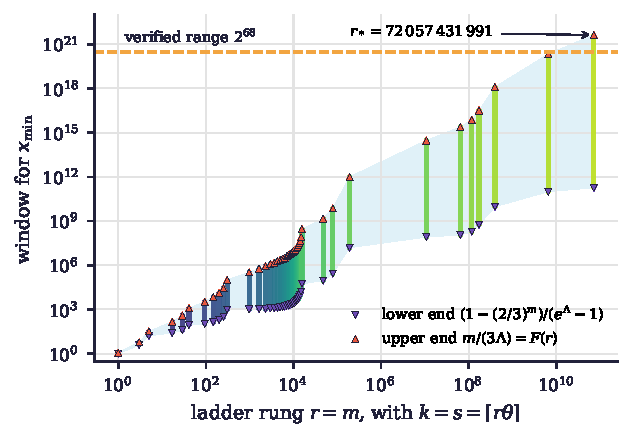
\includegraphics[width=\textwidth]{figures/ch8_window.pdf}
\caption{The window of \cref{lem:ch8:window} for the hypothetical cycles at
every rung of the one sided ladder up to $r_*(2^{68})$. Downward triangles are
the lower ends $(1-(2/3)^m)/(e^\Lambda-1)$, upward triangles the upper ends
$F(m)=m/(3\Lambda)$; the vertical segments are the windows. Only the rung
$r_*=72\,057\,431\,991$ reaches above the verified range $2^{68}$.}
\label{fig:ch8:window}
\end{figure}

\subsection{An exploration of parity words}

To see where actual cycles of rational numbers sit inside the window, we
enumerated all parity words with $m\le20$ ones and
$\lceil m\theta\rceil\le k\le2m$ letters (sampling $10^6$ words when there are
more than $3\times10^6$), computed $x=c_k(w)/(2^k-3^m)$ for each, and recorded
how close $c_k(w)$ comes to a multiple of $D=2^k-3^m$ (script
\texttt{ch08\_window.py}). Every word defines a cycle of $T$ on the rationals
with odd denominator, the rational cycles\index{rational cycles} of Lagarias\index{Lagarias, J. C.}~\cite{lagarias1990}, and
an integer cycle corresponds to $D\mid c_k(w)$. Three observations emerged.

First, the only integer hits for $m\le20$ are the words of the trivial cycle
$\{1,2\}$ repeated, at $k=2m$; this is of course consistent with
\cref{thm:cycles}.
The closest approaches of $c_k(w)/D$ to an integer are of the size predicted by a model in which the residues $c_k(w)\bmod D$ of the words examined are independent and uniform on the nonzero classes: over the $92$ shapes $(m,k)$ with at least $50$ words, the closest approach divided by its expected value under the model has mean $1.1$ and median $0.66$, where the model gives $1$ and about $\log2=0.69$, and the median drifts only from $0.87$ for $m\le12$ to $0.63$ for $m\ge13$ while the expected value itself falls from $8\times10^{-2}$ to $2\times10^{-7}$ (\cref{fig:ch8:words}, right).
We found no sign of a structural obstruction at
this scale, in either direction.

Second, the least element of a rational cycle can sit nearly anywhere in the window:
over all rotation classes with $m\le11$ the ratio of the least element to the
lower end of the window attains $1$ (the lower bound of
\cref{lem:ch8:window} is sharp, attained by the word with all odd steps
first), and the least element never exceeds $0.87$ of the upper end $m/(3\Lambda)$ of its window: the largest ratio, $3\log(4/3)=0.863$, is that of the trivial cycle repeated, and for $k<2m$ the ratio stays below $0.79$, while the harmonic mean of the odd elements, which is what the proof of \cref{lem:ch8:window} actually bounds, reaches $0.995$ of the upper end
(\cref{fig:ch8:words}, left).

Third, for the balanced words\index{balanced words}, the Christoffel words with $m$ ones spread as
evenly as possible among $k$ letters, which are the natural candidates for a
cycle with $k/m$ close to $\theta$, the least and greatest odd elements sit at nearly fixed fractions of the upper end when $k=\lceil m\theta\rceil$: for the $1154$ primitive balanced words ($\gcd(m,k)=1$) with $100\le m\le2000$, $x_{\min}/F(m)$ lies in $[0.719,\,0.724]$ and the greatest odd element in $[1.435,\,1.444]\,F(m)$, close to $1/(2\log2)=0.7213$ and $1/\log2=1.4427$.
(When $\gcd(m,k)>1$ the balanced word is a shorter one repeated and gives the same rational cycle; thus $m=400$ and $800$ repeat $m=200$.)
A heuristic explains the constants. For a balanced word the
odd elements of the cycle are nearly a geometric progression in $\log_2$, filling
an interval $[x_{\min},2x_{\min}]$ with $\log_2x$ nearly uniformly
distributed; then the mean of $1/x_i$ is about
$x_{\min}^{-1}\int_0^12^{-u}\,du=1/(2x_{\min}\log2)$, and
$\Lambda\approx\sum_i1/(3x_i)$ gives $F(m)=m/(3\Lambda)\approx2\log2\,x_{\min}$.
We record this as an observation, not a theorem: it says that for balanced
words the least element sits a fixed fraction below the top of the window, so
balanced words are as far as possible from the factor $m/3$ that
\cref{cor:ch8:window} asks for. Any arithmetic proof that there are no cycles
must therefore treat balanced words by divisibility, not by size.

\begin{figure}[ht]
\centering
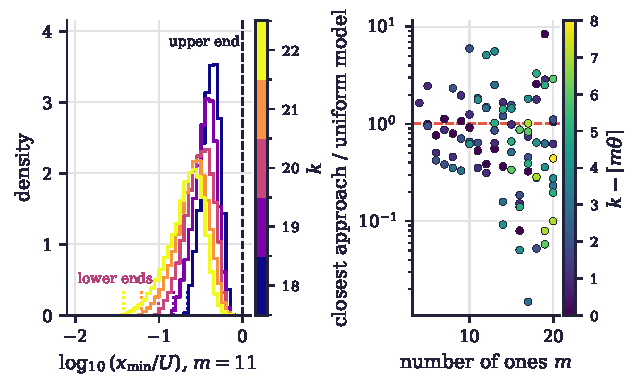
\includegraphics[width=\textwidth]{figures/ch8_words.pdf}
\caption{Left: distribution of $\log_{10}(x_{\min}/U)$, where $U=m/(3\Lambda)$ is the upper end of the window for the given $k$, over rotation classes
of rational cycles with $m=11$, for each $k$ from $\lceil m\theta\rceil=18$ to $2m=22$ (colour); the lower ends
of the windows are marked (dotted). Right: the closest approach of $c_k(w)/D$ to an
integer, relative to its expected value when the residues of the words examined are independent and uniform on the nonzero classes modulo $D$, for the shapes with at least $50$ words, against the number of ones $m$,
coloured by $k-\lceil m\theta\rceil$.}
\label{fig:ch8:words}
\end{figure}

\section{An exact certificate}\label{sec:ch8:certificate}

The bound of \cref{thm:cycles}(ii) was computed in floating point, at $150$ digits.
For a result of this kind it is worth having a certificate\index{certificate} that uses no
floating point at all: a list of integer inequalities that anyone can check,
and that a proof assistant could check. The mediant lemma\index{mediant lemma} and \cref{thm:ch8:onesided} make such a
certificate short, and we have built one (script \texttt{ch08\_certificate.py},
which runs in eleven seconds).

\paragraph{Step 1: an enclosure of $\lt$.} Take the convergents
\[
  \frac ab=\frac{1\,193\,652\,440\,098}{753\,110\,839\,881},\qquad
  \frac{a'}{b'}=\frac{217\,976\,794\,617}{137\,528\,045\,312},
\]
which lie on opposite sides of
$\theta$. The inequalities $2^a<3^b$ and $3^{b'}<2^{a'}$ certify
$a/b<\theta<a'/b'$, an interval of width exactly $1/(bb')=9.65\times10^{-24}$.
The powers are far too large to form, so each comparison is made by enclosing
$3^b$ between $L\cdot2^e$ and $U\cdot2^e$ with $320$ bit integer mantissas,
computed by repeated squaring with downward and upward truncation; every
truncation is itself an integer inequality, and $39$ squarings suffice.

\paragraph{Step 2: an enclosure of $\log2$.} The partial sums of
$\sum_{n\ge1}1/(n2^n)=\log2$ are lower bounds, and adding the tail bound
$1/((N+1)2^N)$ gives upper bounds; we use an enclosure of width
$9\times10^{-30}$. The exclusions in fact survive the crude replacement of
$\log2$ by $69/100$, and the final feasibility check survives $7/10$, which
follow from the sum to $n=7$: $1163/1680>69/100$ and
$1163/1680+1/1024<7/10$.

\paragraph{Step 3: the partial quotients.} The common prefix of the continued
fraction expansions of the two rational endpoints, less its last term, is
certified to be the beginning of the expansion of $\theta$:
\[ [1;1,1,2,2,3,1,5,2,23,2,2,1,1,55,1,4,3,1,1,15,1,9]. \]

\paragraph{Step 4: the rungs.} From these partial quotients the ladder rungs
are generated exactly, $44$ of them up to $72\,057\,431\,991$. For each rung
$u<r_*$ the exclusion $\delta(u)\ge u\varepsilon$ is checked as an inequality
between rationals built from the enclosures, never using more than $248$ bit
integers; the smallest certified margin is $\delta(u)/(u\varepsilon)>1.355$ (true value $1.361$), at
$u=6\,586\,818\,670$.
At $r_*$ itself the opposite inequality is certified from the upper end of the enclosure, $\delta(r_*)<7.97\times10^{-12}$, so that $\delta(r_*)/(r_*\varepsilon)<0.068$ (true value $0.0677$), and the bound is attained by the method.

\paragraph{Step 5: the records.} The enclosures of $\delta$ are certified to
decrease strictly along the rungs, as \cref{thm:ch8:onesided} predicts, a consistency check on the partial quotients; by that theorem the rungs are the records, and with the mediant lemma this certifies that no other $r$
needs checking. As an independent check, an exact integer scan of all
$r\le2\times10^6$ finds exactly the $37$ records predicted by the ladder.

\begin{table}[ht]
\centering\small
\caption{Selected rungs of the certificate at $X=2^{68}$: the rung $u$, its
numerator $s=\lceil u\theta\rceil$, a certified bound for $\delta(u)$ (a lower bound for $u<r_*$, an upper bound at $u=r_*$),
and the margin $\delta(u)/(u\varepsilon)$, which must exceed $1$ for
exclusion.}
\label{tab:ch8:certificate}
\begin{tabular}{@{}rrcr@{}}
\toprule
$u$ & $s$ & $\delta(u)$ & margin \\
\midrule
$15\,601$ & $24\,727$ & $>2.62\times10^{-5}$ & $>1.0\times10^{12}$ \\
$190\,537$ & $301\,994$ & $>9.30\times10^{-8}$ & $>2.99\times10^{8}$ \\
$10\,781\,274$ & $17\,087\,915$ & $>1.76\times10^{-8}$ & $>1.0\times10^{6}$ \\
$171\,928\,773$ & $272\,500\,658$ & $>2.58\times10^{-9}$ & $>9214$ \\
$397\,573\,379$ & $630\,138\,897$ & $>1.52\times10^{-10}$ & $>235.7$ \\
$6\,586\,818\,670$ & $10\,439\,860\,591$ & $>1.45\times10^{-11}$ & $>1.355$ \\
$72\,057\,431\,991$ & $114\,208\,327\,604$ & $<7.97\times10^{-12}$ & $<0.068$ \\
\bottomrule
\end{tabular}
\end{table}

The certificate is the bridge to a machine checked proof
(\cref{sec:ch8:lean}): every step is an inequality between integers of at
most a few hundred bits, plus two exponentiations handled by a verified
squaring routine.

\section{A sibling problem: Erd\H{o}s 125}\label{sec:ch8:erdos}

Good rational approximations\index{Diophantine approximation} to $\theta$, the raw material of the previous sections, appear in a different role
in a problem from the Erd\H{o}s collection that was settled in 2026.

\subsection{The problem}

Let $A$ be the set of nonnegative integers whose base $3$ digits all lie in
$\{0,1\}$, and $B$ the set of nonnegative integers whose base $4$ digits all
lie in $\{0,1\}$. Then $|A\cap[0,3^n-1]|=2^n$ and $|B\cap[0,4^n-1]|=2^n$, so
$|A\cap[0,N]|$ is of order $N^{\log2/\log3}=N^{0.631}$ and $|B\cap[0,N]|$ of
order $N^{1/2}$. The number of pairs $(a,b)$ with $a+b\leq N$ is therefore of
order $N^{1.131}$, which exceeds $N$ by a power, and positive density of the
sumset $A+B$ is the naive guess. Burr\index{Burr, S. A.}, Erd\H{o}s\index{Erdos, P.@Erd\H{o}s, P.}, Graham\index{Graham, R. L.} and
Li\index{Li, W. W.}~\cite{burr1996} asked whether $A+B$ has positive density; in the form recorded as problem $125$ of the Erd\H{o}s problem collection, the question is whether it has positive lower density.
Melfi\index{Melfi, G.}~\cite{melfi2001} proved that
$|(A+B)\cap[1,x]|\gg x^{0.965}$, and Hasler\index{Hasler, M. F.} and Melfi~\cite{haslermelfi2024} improved the exponent to
$0.97777$ and showed that the lower density is at most
$1015/1458=0.696$.

In 2026 the question was settled negatively by AlphaProof Nexus\index{AlphaProof Nexus}, an agent
that searches for proofs in the Lean\index{Lean} proof assistant, developed at Google
DeepMind by Tsoukalas\index{Tsoukalas, G.}, Kovsharov\index{Kovsharov, A.}, Shirobokov\index{Shirobokov, S.}, Surina\index{Surina, A.} and
collaborators~\cite{tsoukalas2026}: the lower density of $A+B$ is zero. The
same work reports that the agent solved $9$ of $353$ open Erd\H{o}s
problems (formalized in Lean) and $44$ of $492$ conjectures from the OEIS. The proof proceeds by
thinning along windows in which a power of $3$ is close to a power of $4$,
that is, along good rational approximations to the ratio
$\log4/\log3=2/\theta$; an
early very good one is $3^{53}\approx4^{42}$, with ratio $1.0021$. DeepMind's
work does not address the Collatz problem; the link we draw is through this
Diophantine\index{Diophantine approximation} mechanism.

\subsection{An exact computation}

We computed the counting function $|(A+B)\cap[0,N]|$ exactly for every
$N\leq4^{13}=67\,108\,864$, by marking each sum $a+b\leq N$ in a bit array, as
reported in our note~\cite{polsonsokolov2026nexus}. For this chapter we reran
the computation independently (script \texttt{ch08\_erdos125.py}; the run to
$4^{13}$ takes about sixteen seconds) and reproduced every entry of
\cref{tab:ch8:erdos} to the four digits shown, as well as the location and
value of the minimum.

\begin{table}[ht]
\centering
\caption{Density $|(A+B)\cap[0,N]|/(N+1)$ at powers of $4$ and of $3$. The
exact minimum over $10^4\leq N\leq4^{13}$ is $0.763392$, at
$N=3^{15}-1=14\,348\,906$.}
\label{tab:ch8:erdos}
\begin{tabular}{@{}lllll@{}}
\toprule
$N$ & density & \qquad & $N$ & density \\
\midrule
$4^{7}$ & $0.8593$ && $3^{10}$ & $0.7785$ \\
$4^{8}$ & $0.7913$ && $3^{11}$ & $0.8372$ \\
$4^{9}$ & $0.8372$ && $3^{12}$ & $0.8583$ \\
$4^{10}$ & $0.8688$ && $3^{13}$ & $0.8742$ \\
$4^{11}$ & $0.8068$ && $3^{14}$ & $0.8147$ \\
$4^{12}$ & $0.7836$ && $3^{15}$ & $0.7634$ \\
$4^{13}$ & $0.8382$ && $3^{16}$ & $0.8312$ \\
\bottomrule
\end{tabular}
\end{table}

\begin{figure}[ht]
\centering
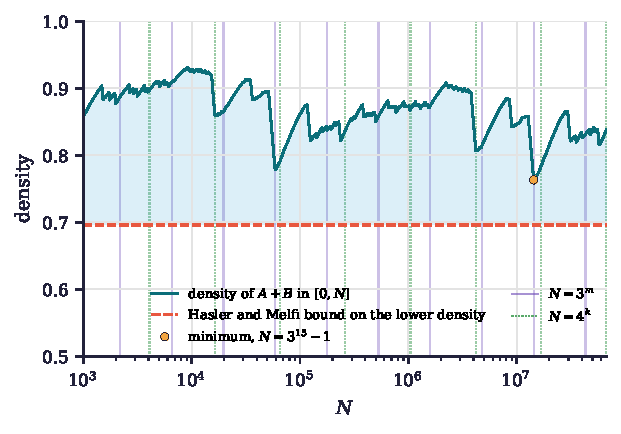
\includegraphics[width=\textwidth]{figures/ch8_erdos125.pdf}
\caption{Density of $A+B$ in $[0,N]$ for $10^3\leq N\leq4^{13}$, with
vertical lines at the powers of $3$ (solid) and of $4$ (dotted) and the Hasler and Melfi upper bound
$1015/1458$ on the lower density.}
\label{fig:ch8:erdos}
\end{figure}

Three things are visible in \cref{fig:ch8:erdos}. The density stays well above
the Hasler and Melfi bound throughout the range, so finite computation gives
no hint that the lower density is zero: the decay that the proof exploits
operates at the scale of the good approximations to $2/\theta$, and the first
very good one, $3^{53}\approx4^{42}$, is far beyond any computation. The
minima sit just below powers of $3$, where a new block of $A$ is about to
begin and the previous blocks have been exhausted. And the deepest dips occur
when a power of $3$ lies a little below a power of $4$: $3^{10}/4^{8}=0.90$
and $3^{15}/4^{12}=0.855$ are such cases, and they give the two lowest values
in the table. This is the thinning mechanism of the proof seen at small scale:
when $3^m$ and $4^k$ are close, the two digit structures align, and the gaps
of $A$ and of $B$ overlap rather than fill each other.

\subsection{The analogy}

Both problems turn on good rational approximations to a ratio of logarithms, but they use them in opposite ways.
For Erd\H{o}s $125$ the coincidences are $3^m\approx4^k=2^{2k}$, that is, approximations $2k/m$ to $\theta$ from either side; they produce windows in which $A+B$ thins, and the proof uses infinitely many such windows to drive the lower density to zero.
Only their existence matters, and it follows from soft arguments, such as the pigeonhole principle or \cref{lem:ch8:basic}; the example $3^{53}\approx4^{42}$ is the convergent $84/53$, which lies below $\theta$ and is useless for cycles (\cref{rem:ch8:false}).
For Collatz cycles the good approximations $3^r\approx2^s$ with $s/r$ just above $\theta$ are exactly what a cycle needs; their records bound the length of a cycle (\cref{thm:cycles}), but by \cref{prop:ch8:insufficient} they are good enough infinitely often, whatever the verification range, so no information about the approximations of $\theta$ alone, not even bounded partial quotients, can exclude every cycle.
In one problem the existence of good approximations is the engine of the proof; in the other it is an obstruction that Diophantine\index{Diophantine approximation} approximation cannot remove, and what is missing is arithmetic information about the parity word (\cref{cor:ch8:window}).
That asymmetry is a fair summary of why the cycle half is hard.

\section{Machine checked statements}\label{sec:ch8:lean}

A bound such as \cref{thm:cycles} is assembled from a short chain of
elementary steps and a finite computation, which makes it an attractive
target for formal verification. In our note~\cite{polsonsokolov2026nexus} we
wrote two small files in Lean\index{Lean}~4~\cite{moura2021}, using only the core library
(Lean 4.15, without Mathlib). The restriction is severe: there are no real
numbers, no rationals and no limits, so every statement must be phrased in
natural number arithmetic, and every proof uses only induction, case
analysis, linear arithmetic and the kernel. It is also useful, since it
forces exactly the logarithm free formulations a verified cycle bound will
need. Both files compile; the first produces no warnings, the second one
warning for each open statement. They are in the folder \texttt{lean} of the book's repository (\cref{app:code}).

\lstdefinestyle{ch8lean}{language={},basicstyle=\ttfamily\scriptsize,literate={→}{{$\to$}}1 {∃}{{$\exists$}}1 {∀}{{$\forall$}}1 {∧}{{$\land$}}1 {∨}{{$\lor$}}1 {¬}{{$\neg$}}1 {≤}{{$\le$}}1 {≥}{{$\ge$}}1}

\subsection{What is proved}

The definitions are the accelerated map\index{accelerated map}, its iterates and the number of odd
steps.

\begin{lstlisting}[style=ch8lean]
def T (x : Nat) : Nat :=
  if x % 2 = 0 then x / 2 else (3 * x + 1) / 2
def Tn : Nat → Nat → Nat
  | 0, x => x
  | k + 1, x => T (Tn k x)
def odd : Nat → Nat → Nat
  | 0, _ => 0
  | k + 1, x => odd k x + (if Tn k x % 2 = 1 then 1 else 0)
\end{lstlisting}

\noindent The four theorems are the following.

\begin{lstlisting}[style=ch8lean]
theorem B1 (k x : Nat) : ∃ c : Nat,
    2 ^ k * Tn k x = 3 ^ (odd k x) * x + c ∧
    (odd k x > 0 → c > 0)
theorem B2 {k x : Nat} (hx : x > 0) (hk : k > 0)
    (hcyc : Tn k x = x) (ho : odd k x > 0) :
    3 ^ (odd k x) < 2 ^ k
theorem B3 : ∀ x, 1 ≤ x → x ≤ 10000 →
    ∃ j, j ≤ 400 ∧ Tn j x = 1
theorem B4 : Tn 1 1 = 2 ∧ Tn 2 1 = 1 ∧
    ∀ k, Tn k 1 = 1 ∨ Tn k 1 = 2
\end{lstlisting}

B1 is the affine identity of \cref{prop:ch2:affine}, proved by induction on
$k$ through a stronger lemma that names the remainder by the explicit
recursion $c_{k+1}=3c_k+2^k$ after an odd step and $c_{k+1}=c_k$ after an even
one; an inductive hypothesis asserting only the existence of some remainder is
awkward to propagate. B2 is the cycle inequality $3^m<2^k$ of
\cref{cor:ch2:cycle}, the lower half of \eqref{eq:ch8:theta}. B3 checks that
every starting value from $1$ to $10^4$ reaches $1$ within $400$ steps of $T$
(the true maximum is $165$ steps, at $x=6171$, by our own count). It starts at
$x=1$ because $0$ is a fixed point of $T$, so the statement over all
$x\leq10^4$ would be false. It is proved by a Boolean evaluator together with
a kernel checked soundness lemma, and the evaluation is run natively rather
than in the kernel, so the proof depends on the axiom
\texttt{Lean.ofReduceBool}, which amounts to trusting the compiled evaluator.
B4 describes the trivial cycle. The axiom report printed by Lean\index{Lean} is: B1 uses
\texttt{propext} and \texttt{Quot.sound}; B2 also uses
\texttt{Classical.choice}; B3 uses \texttt{propext}, \texttt{Quot.sound} and \texttt{Lean.ofReduceBool}; B4 uses no
axioms. The proofs were written by an AI coding agent working against the
compiler, and we then recompiled both files independently and read every
statement against its informal meaning, which is where the two details just
mentioned were caught.

\subsection{What is stated}

The open statements are the conjecture, its descent form, and the cycle
problem.

\begin{lstlisting}[style=ch8lean]
theorem O1_collatz : ∀ x, x ≥ 1 → ∃ k, Tn k x = 1
theorem O3_descent : ∀ x, x ≥ 2 → ∃ k, k > 0 ∧ Tn k x < x
theorem O4_no_cycles : ¬ ∃ x k, x > 2 ∧ k > 0 ∧ Tn k x = x
\end{lstlisting}

\noindent The names O1, O3 and O4 are those of the Lean files and are unrelated to the numbering of the problems in \cref{chap:open}.
O3 implies O1 by strong induction, and O1 implies O3 because an orbit that
reaches $1$ passes below its starting value. O4 excludes every cycle of
positive integers other than $\{1,2\}$; the hypothesis $x>2$ rules out the
elements of the trivial cycle, and $x=0$ is excluded with them.

\subsection{From statements to a verified cycle bound}

What separates these files from a verified form of \cref{thm:cycles} is the
upper half of \eqref{eq:ch8:theta} and the continued fraction\index{continued fraction} computation.
Both are within reach of the core library once they are stated without
logarithms. For the first, if every element of a cycle of $T$ with $k$ steps
and $m$ odd steps is at least $X$, then by \eqref{eq:ch8:prod}
\[
  2^k=\prod_{i=1}^{m}\Bigl(3+\frac1{x_i}\Bigr)\leq\Bigl(3+\frac1X\Bigr)^m,
  \quad\text{that is}\quad 2^k(3X)^m\leq3^m(3X+1)^m,
\]
an inequality between natural numbers which, combined with B2, is the whole
content of \cref{lem:cycleid} and \cref{cor:ch8:excl}.

For the second, the exclusion of all $m<r_*(X)$ can be replaced by the short
certificate\index{certificate} of \cref{sec:ch8:certificate}. The proof of \cref{thm:cycles}(ii) uses three ingredients: the
identities of \cref{lem:ch8:basic}(ii) for the listed pairs $(p_i,q_i)$ of convergents, which
are integer arithmetic; the signs of $q_i\theta-p_i$, which are comparisons
between $3^{q_i}$ and $2^{p_i}$; and, at each rung $u$, the inequality
$\delta(u)\geq u\varepsilon$. Checking a comparison such as
$3^{q}$ against $2^{p}$ for $q$ near $10^{11}$ by direct exponentiation is
out of the question, but interval arithmetic on rational approximations of
$\lt$, proved once, reduces each check to arithmetic on integers of modest
size, as in Steps 1 to 4 of \cref{sec:ch8:certificate}; since the quantities $\delta(u)$ involved are of order $10^{-11}$ and
the margins are at least a factor $1.36$, a rational enclosure of $\lt$ to a
few dozen digits suffices.
The mediant lemma\index{mediant lemma} and \cref{thm:ch8:onesided} keep the certificate short: instead of checking $\delta(m)\geq m\varepsilon$ for each of the some $7\times10^{10}$ values $m<r_*$, \cref{cor:ch8:firstfeasible} and the lattice argument of
\cref{thm:ch8:onesided} reduce the task to the $44$ rungs up to
$r_*(2^{68})$, and there are only $53$ rungs below $2\times10^{13}$ in all.
This is a well posed task for an automated prover of the AlphaProof Nexus\index{AlphaProof Nexus}
type, and it would make the cycle bound the first part of the programme of
this book to be fully machine checked. The remaining trusted input would be
the verification range\index{verification range} itself, which rests on a large computation of a
different kind.

\section{A refined open problem}\label{sec:ch8:refined}

The cycle length bounds above use the cycle structure only through the crude inequality $\log(1+1/(3x_i))\leq1/(3M)$, and the window lemma adds only the lower bound $c_k\geq3^m-2^m$.
For any cycle with $m$ odd steps, $k$ steps in all and smallest element $x_{\min}$, \cref{lem:ch8:window} gives
\[
  x_{\min}<\frac{m}{3\Lambda}\le\frac{m}{3\log2\;\delta(m)},\qquad\Lambda=k\log2-m\log3 .
\]
The remaining information in a cycle lies in its parity vector\index{parity vector}. A cycle of $T$
is described by a word of length $k$ with $m$ ones, and by
\cref{cor:ch2:cycle} each element is $x=c_k(x)/(2^k-3^m)$, where the affine
constant $c_k(x)$ of \eqref{eq:ch2:cexplicit} is a sum of terms $3^{j}2^{i}$
indexed by the positions of the ones in the word. The thinning argument of the
Erd\H{o}s $125$ proof controls how two digit expansions interact over a window
in which $3^m\approx4^k$, and it is natural to ask whether a similar block
decomposition of the parity word can be brought to bear here.

\begin{problem*}[Arithmetic sharpening of the cycle identity]
Find a function $f$, derived from the arithmetic of the parity vector rather
than from the size of the elements, such that every nontrivial cycle with $m$
odd steps and $k$ steps in all satisfies
\[
  x_{\min}<\frac{m}{3\Lambda\,f(m)},\qquad\Lambda=k\log2-m\log3 .
\]
By \cref{cor:ch8:window}, any $f$ with $f(m)\geq\frac m3(1+\eta)$ for large $m$ would confine the least element of every nontrivial cycle with many odd steps below about $1/(2\eta)$, and so reduce the cycle half to a finite verification; one may also try to raise the lower end $(1-(2/3)^m)/(e^{\Lambda}-1)$ of the window by a factor slightly more than $m/3$, which would empty the window whenever $\Lambda$ is small.
More concretely: does a block decomposition of the parity word, in
the style of the thinning argument for Erd\H{o}s $125$, force $c_k(x)$ to be
large compared with $3^m-2^m$, or constrain it modulo $2^k-3^m$, in a way that
the size of $x$ alone does not?
\end{problem*}

The target is demanding. For balanced words\index{balanced words} the least element already sits at
about $0.72$ of the upper end of the window, so no size argument can gain the
factor $m/3$ there, and the exploration of parity words found residues
$c_k(w)\bmod(2^k-3^m)$ behaving like uniform random variables. A proof along
these lines must therefore exploit divisibility, and would amount to showing
that $2^k-3^m$ never divides $c_k(w)$ except for the trivial word. Any partial
result with $f$ bounded below by a constant $b>1$ would lower every threshold of \cref{tab:ch8:thresholds} by at least the factor $b$, which is worth at least as much as a verification range larger by the factor $b$, at every range at once; a result with $f(m)\to\infty$ would eventually gain more than any fixed increase of the verification range. We collect the problem, with the others raised in the book, in
\cref{chap:open}.

\section*{Notes}

The cycle identity\index{cycle identity} and the bound $M<r/(3\Lambda_r)$ go back at least to the
1970s; the use of continued fractions\index{continued fraction} of $\lt$ for cycle bounds is due to
Crandall\index{Crandall, R. E.}~\cite{crandall1978}, whose criterion is in substance the block bound of \cref{lem:block}, to
Steiner\index{Steiner, R. P.}~\cite{steiner1977} and, with larger verification ranges\index{verification range}, to
Eliahou\index{Eliahou, S.}~\cite{eliahou1993}. The surveys of Lagarias\index{Lagarias, J. C.}~\cite{lagarias1985} and
the collection~\cite{lagarias2010} describe the history, including the
negative cycles\index{negative cycles} and the $3x-1$ problem, and Lagarias~\cite{lagarias1990}
treats the rational cycles\index{rational cycles}. Simons and de Weger~\cite{simons2005} and
Hercher\index{Hercher, C.}~\cite{hercher2023} are the current state of the art for $m$ cycles
and for the length bound, Hercher's record~\cite[Corollary~29]{hercher2023} being unconditional since the verification to $2^{71}$. The verification ranges $2^{68}$ and $2^{71}$ are due to
Ba\v{r}ina\index{Barina, D.@Ba\v{r}ina, D.}~\cite{barina2021,barina2025}; see also the account of earlier verification
efforts in~\cite{lagarias2010}. For continued fractions,
Khinchin~\cite{khinchin1964} remains the most economical introduction, Hardy
and Wright~\cite{hardywright2008} give the best approximation theorems, and
Rockett and Sz\"usz~\cite{rockett1992} treat one sided approximation\index{one sided approximation} and the
role of the intermediate fractions\index{semiconvergent}. Linear forms in two logarithms are treated
by Laurent, Mignotte and Nesterenko~\cite{laurent1995}, and the general theory
by Baker~\cite{baker1975}. The record structure of \cref{prop:records} is classical, equivalent to finding
the least denominator fraction in an interval just above $\lt$ (Lemma 22 of
Hercher~\cite{hercher2023}), and is the description of the best one sided approximations that Han\v{c}l\index{Hancl, J.@Han\v{c}l, J.} and Turek\index{Turek, O.}~\cite[Theorem~4.5(ii)]{hancl2019} state and prove; the mediant lemma\index{mediant lemma} and \cref{thm:ch8:onesided} give a short self contained proof of the
part we need. Halbeisen\index{Halbeisen, L.} and Hungerb\"uhler\index{Hungerbuhler, N.@Hungerb\"uhler, N.}~\cite{halbeisen1997} give the optimal criterion, attained by the balanced parity word, and observe for Eliahou's criterion that the dangerous lengths lie between convergents, that convergents from the wrong side are harmless and that multiples tie exactly~\cite[\S4.4]{halbeisen1997}. The comparison of exact and crude bounds, the integer
certificate\index{certificate}, the threshold table, the insufficiency proposition and the window
corollary are ours, although the structural point of the insufficiency proposition is made in another form in~\cite[\S5]{halbeisen1997}; the lower bound
$c_k\geq3^m-2^m$ underlying the window is elementary and is implicit in the
classical analyses of cycles by B\"ohm\index{Bohm, C.@B\"ohm, C.} and Sontacchi\index{Sontacchi, G.}~\cite{bohm1978} and by Steiner. The Erd\H{o}s $125$ problem is from Burr, Erd\H{o}s, Graham
and Li~\cite{burr1996}, and its resolution is in Tsoukalas and
collaborators~\cite{tsoukalas2026}; the exact density computation and the Lean\index{Lean}
files are from our unpublished note~\cite{polsonsokolov2026nexus}. For Lean~4 see de Moura\index{de Moura, L.}
and Ullrich\index{Ullrich, S.}~\cite{moura2021}.

\section*{Exercises}

\begin{exercise}
Verify the cycle identity\index{cycle identity} \eqref{eq:ch8:prod} for the three negative cycles\index{negative cycles} of
\cref{tab:ch8:negative}, and show that for a cycle of negative integers the
inequality is reversed: $2^s<3^r$. Show that the conjugation $n\mapsto-n$
carries $T_0$ on the negative integers to the map $n\mapsto n/2$ ($n$ even),
$n\mapsto3n-1$ ($n$ odd) on the positive integers, and list the corresponding
cycles of this map.
\end{exercise}

\begin{exercise}
Using \eqref{eq:ch2:affine}, find the rational periodic points of $T$ whose
parity words are $(1,0)$, $(1,1,0)$, $(1,0,0)$ and $(1,1,0,0)$, and check
which of them are integers. Show that for every word $w$ with $2^k\neq3^m$ the
number $c(w)/(2^k-3^m)$ is a rational number with odd denominator whose orbit
under $T$ is periodic with parity word $w$.
\end{exercise}

\begin{exercise}
Prove that the best approximations from below, the $r$ with
$\{r\theta\}<\{r'\theta\}$ for every $1\leq r'<r$, are exactly $r=1$ and the rungs
$q_{k-1}+jq_k$ with $k\geq1$ odd and $1\leq j\leq a_{k+1}$, by adapting the proof
of \cref{thm:ch8:onesided}. List them for $\lt$ below $700$.
\end{exercise}

\begin{exercise}
Show that if $q$ is a rung and $t\geq2$ is an integer with $t\,\delta(q)<1$,
then $\delta(tq)=t\,\delta(q)$ and $F(tq)=F(q)$. Deduce directly, without the
mediant lemma\index{mediant lemma}, that $tq$ is never a strict record of $F$. Which multiples of
$q_9=15\,601$ satisfy the hypothesis?
\end{exercise}

\begin{exercise}
Show that for even $i\geq0$ one has $\delta(q_i)=1-\varepsilon_i$, so that $F(q_i)=q_i/(3(1-\varepsilon_i)\log2)$, only slightly more than $q_i/(3\log2)$, and explain the triangles of \cref{fig:ch8:records}. Then, for a cycle of $T$ with $k$ steps and $m$ odd steps all of whose elements are at least $X$, prove the logarithm free inequality $2^k(3X)^m\leq3^m(3X+1)^m$, and deduce from it and $\log(1+u)<u$ for $u>0$ that $\delta(m)<m/(3X\log2)$.
\end{exercise}

\begin{exercise}
For the Erd\H{o}s $125$ sets, prove that $|A\cap[0,3^n-1]|=|B\cap[0,4^n-1]|=2^n$
and that the number of pairs $(a,b)\in A\times B$ with $a+b\leq N$ is of order
$N^{\log2/\log3+1/2}$. Using \texttt{ch08\_erdos125.py} or your own code,
compute the density of $A+B$ in $[0,N]$ for $N=3^m-1$ and $N=4^k$ up to
$4^{10}$, and relate the depth of each dip to the ratio $3^m/4^k$ for the
nearest powers.
\end{exercise}

\begin{exercise}
Show that the lower bound of \cref{lem:ch8:window} is attained exactly by the
rotation of a parity word whose $m$ ones come first, and compute the window for
$m=2$, $k=4$. Is there an integer in it? Which rational cycle\index{rational cycles} sits at its lower
end?
\end{exercise}

\begin{exercise}
Let $\nu=2$ and suppose $|\lt-s/r|\geq c/r^2$ for all $r$. Show that the
verification range\index{verification range} $X$ then excludes exactly the $r<(3cX\log2)^{1/2}$ that the
inequality \eqref{eq:ch8:irrbound} can handle, and that \cref{prop:ch8:insufficient}
still produces infinitely many nonexcluded $r$. Conclude that bounded partial
quotients for $\lt$ would not by themselves exclude all cycles.
\end{exercise}

